\documentclass[10pt]{article}
%\renewcommand{\baselinestretch}{0.975}
\usepackage{latex8}
\usepackage{times}
\usepackage{graphicx}
\usepackage[usenames,dvipsnames,svgnames,table]{xcolor}
\usepackage{tabularx}
\usepackage[T1]{fontenc}
\usepackage{verbatim}
\usepackage{enumerate}
\usepackage{amsmath,amssymb}
\usepackage{pdfpages}
\usepackage{amsthm}
\usepackage{subcaption}
\usepackage{tikz}
%\usetikzlibrary{timeline}
\usepackage{wrapfig}
\usepackage{pdfpages}
\usepackage{xsavebox}
\newtheorem{theorem}{Theorem}
\newtheorem{lemma}{Lemma}
\setcounter{lemma}{0}
\newtheorem{defin}{Definition}
\setcounter{defin}{0}
% table of contents
\usepackage{hyperref}
\hypersetup{colorlinks=true,allcolors=blue}
\usepackage{hypcap}
\usepackage{multirow}

%dummy text
\usepackage[english]{babel}
\usepackage{blindtext}
\usepackage{longtable}
\usepackage{booktabs}
\usepackage[table]{xcolor}
\usepackage{pgfgantt}
\usepackage{fancyvrb}
\usepackage{array}
\usepackage{hhline}
\usepackage[math]{cellspace}
\usepackage{mathtools}
\usepackage{cite}
\usetikzlibrary{positioning}

\cellspacetoplimit 4pt
\cellspacebottomlimit 4pt
\newcommand{\ignore}[2]{\hspace{0in}#2}
\newcommand*{\tabulardef}[3]{\begin{tabular}[t]{@{}m{1.75cm}m{\dimexpr\linewidth-#1}@{}}
    #2 & #3
  \end{tabular}}
\newcommand{\simincom}[1]{\textcolor[rgb]{0.87,0.28,0.00}{\noindent$<$\textbf{Nesredin: }\textit{#1}$>$}}
\newcommand{\dagcom}[1]{\textcolor[rgb]{0.87,0.28,0.00}{\noindent$<$\textbf{Cristina: }\textit{#1}$>$}}

\graphicspath{ {pics/} }

% research goals Commands
\newcommand{\og}[1]{\paragraph{Overall goal: }~\parbox[c]{0.7\textwidth}{#1}\\}
\newcounter{rgcounter}
\newcommand{\rg}{%
\stepcounter{rgcounter}%
Research Goal \thergcounter: }

% research contribution command
\newcounter{rccounter}
\newcommand{\rc}{%
\stepcounter{rccounter}%
Contribution \therccounter}
\newcommand{\cc}[1]{%
\stepcounter{rccounter}%
\paragraph{Contribution \therccounter:}\parbox[c]{0.7\textwidth}{#1}\\}

\newcommand{\ogl}[1]{
Overall Goal:
\fcolorbox{gray}{light-gray}{
          \begin{minipage}[t]{0.7\textwidth}
    #1
    \end{minipage}}
}
\newcommand{\rgl}[1]{
\rg
\fcolorbox{gray}{light-gray}{
          \begin{minipage}[t]{0.7\textwidth}
    #1
    \end{minipage}}
}
\usetikzlibrary{external}
% \tikzexternalize[mode=list and make]
\tikzset{
    png export/.style={
        % First we call ImageMagick; change settings to requirements
        external/system call/.add={}{; convert -density 300 -transparent white "\image.pdf" "\image.png"},
        % Now we force the PNG figure to be used instead of the PDF
        /pgf/images/external info,
        /pgf/images/include external/.code={
            \includegraphics[width=\pgfexternalwidth,height=\pgfexternalheight]{##1.png}
        },
    }
}


\definecolor{light-gray}{gray}{0.95}
\newenvironment{researchgoal}
{\begin{center}}
{\end{center}}
% papers command
\newcommand{\pp}{Paper cont.}
\DeclarePairedDelimiter{\ceil}{\lceil}{\rceil}
\begin{document}

%-------------------------------------------------------------------------
% take the % away on next line to produce the final camera-ready version
%\pagestyle{empty}

%-------------------------------------------------------------------------
\begin{center}
\vspace{4cm}

\LARGE \textbf {DOCTORAL THESIS PROPOSAL} \\[3cm]

%\LARGE \textbf {Developing Data Aggregation Support for Real-Time Applications} \\[2cm]
\LARGE \textbf {Design of Assured and Efficient Safety-critical Embedded Systems} \\[2cm]

\normalsize{Nesredin Mahmud } \\
School of Innovation, Design and Engineering (IDT) \\
M\"{a}lardalen University \\
nesredin.mahmud@mdh.se \\
October 2018\\

\vspace{3cm}

\begin{minipage}{1.0\textwidth}
	\begin{flushright} \small
		\textbf{Main Supervisor: Cristina Seceleanu} \\
		\textbf{Co-supervisor: Guillermo Rodriguez-Navas}
	\end{flushright}
\end{minipage}

\vfill

%empty page after the title

\end{center}

\newpage

% abstract page
\begin{abstract}
Safety-critical systems have to fulfill functional, timing and reliability requirements, which makes their design particularly challenging. In fact, several safety standards including ISO 26262 for the automotive domain,  MIL-STD-2167/DO-178C for avionics, etc., recommend systematic processes and techniques to be applied at various stages of system development.  In order to minimize cost and improve software quality, systems should be analyzed at earlier stages before implementation. Model-based development and formal techniques are promising solutions in this regard and have been employed to manage complexity and to analyze system abstractions at early development stages. Nevertheless, the application of formal techniques has been limited in practice mainly due to technical challenges such as their scalability and usability. 

The research presented in this thesis provides formal techniques and tools to address the above challenges during requirements specification, software design, and software allocation phases of multirate embedded systems. In multirate systems, certain operations must be executed periodically, and each operation is executed at its own rate. Specifically, the multiple sampling times cause various timed paths of signal propagation in the software application, thus resulting in different delay semantics (or interpretations). Multirate designs are frequently employed in automotive, industrial automation, avionics domains. 

To address the requirements phase, in the thesis we propose a domain-specific requirements specification language called ReSA, as well as consistency checking techniques in order to improve specifications, before their use in system design and implementation. During the system design phase, system designs are refined via software design units often specified in Simulink, which is a graphical programming environment for modeling and analyzing multidomain systems, which is frequently employed in industry. To check that Simulink designs conform to the system's functional and timing requirements, while addressing scalability, we provide a formal analysis technique of the former via statistical model checking. The method relies on patterns that formalize discrete- and continuous-time Simulink blocks into stochastic timed automata, while preserving the block execution order generated by Simulink. Next, we also provide integer-linear-programming-based allocation methods of software applications, to optimize power consumption of multirate systems while guaranteeing satisfiability of timing and reliability requirements, and design and hardware constraints. To automate the above steps, we also propose tools for requirements specification and analysis, as well as for the transformation of Simulink models into stochastic timed automata networks for statistical model checking. Our proposed methods and tools are validated on automotive industrial use cases. 
\end{abstract}

\newpage
\tableofcontents
\newpage

\section{Introduction}
\label{section:introduction}
%% what is the area of the research
% - topic: software development/design/analysis
% - domains: automotive, aeronautics, ..
% - areas: iot, embedded systems, cyber-physical, distributes systems...
% - methods: model-based development, formal methods, ...
% - problems: increasing complexity, stringent standards, market competitiveness, compatibility

An embedded system is some combination of computer hardware and software, either fixed in capability or programmable, placed within a larger system. Industrial machines, automobiles, medical equipment, airplanes, vending machines, as well as mobile devices are all possible locations for an embedded system  \cite{WangJiacun2017RES}. In contrast to traditional software systems, e.g., web applications, desktop applications, embedded systems are usually safety critical, which means their failure to operate properly could cause fatalities and immense properties damage. Moreover, they operate in a rogue environment without interruption for a long time, therefore such systems should be dependable in many ways, for instance, they must be timely and reliable. The hardware platforms on which embedded software programs execute are resource constrained, therefore, efficient software partitioning and deployment is crucial especially in the midst of increasing software applications and their increasing functional complexity. In fact, the development of safety-critical embedded systems is driven by stringent functional safety requirements from respective industry standards, e.g., ISO 26262  in automotive systems \cite{iso201126262}, MIL-STD-2167/DO-178C in avionics \cite{Wang2016DevelopingDO-178Cb}, IEC 61511 in process engineering \cite{bond2002iec}, etc, in order to ensure the quality of embedded systems, which is required to be enforced at different levels, including system development, maintenance, and operation. For instance, the ISO 26262 standard for automotive systems highly recommends rigorous methods to specify and analyze the systems, by applying \textit{formal methods} at different levels of system development, such as requirements specification, system design and implementation. Formal methods \cite{OreganUndergraduateScience} are mathematical techniques that can help the specification and analysis of system models, with precision and without ambiguity. In particular, in this thesis, we apply \textit{lightweight formal methods} \cite{lightweigh2001,Agerholm1999AMethods}, which tackle the difficulty of applying formal methods by applying partial specification, modeling, and focused analysis of relevant system parts, thereby facilitating their applicability in practice. 
\begin{figure}[h!]
  \centering
  \begin{subfigure}[b]{0.575\linewidth}
  \includegraphics[width=\linewidth]{multirate}
  \caption{Brake-By-Wire Block Diagram.}
     \label{fig_smultirate}
  \end{subfigure}\vspace{-0.05cm}
  \begin{subfigure}[b]{0.4\linewidth}
    \includegraphics[width=\linewidth]{pics/timedpath.pdf}
    \caption{Timed Paths for the Chain: {\small ABS\_RR\_Whl (t1)$\rightarrow$ Vehile\_Body\_Whl  (t2)$\rightarrow$ Vehile\_Spd\_Estimator  (t3)}.}
    \label{fig_timedpath}
  \end{subfigure}
  \caption{Multirate System, Brake-By-Wire Example.}
  \label{fig_multirate}
\end{figure}

The difficulty of satisfying the timing requirements of embedded systems increases especially when embedded software applications are designed to run over different sampling times (or activation patterns), also known as \textit{multirate}. A multriate design approach enables multitasking by allowing the tasks that realize the functionalities of software applications to execute independently (that is on their own sample time) through interleaving. The timing analysis of multirate systems is complex due the various timed paths that are generated as signals propagate from the sourcing tasks to the sinking tasks. The timed paths are interpreted according to various delay semantics of which the most common are age delay and reaction delay. 
\cite{Feiertag2009ASemantics,mubeen2013support,Becker2017End-to-endSystems}. Multirate designs are widely observed in embedded systems, including in the automotive domain. 

Assuming a Brake-by-Wire (BBW) system that controls the brakes of a car through electrical means, in Figure \ref{fig_smultirate} we show a software application model for the specific part of the BBW system in which the rear-wheel rotation speed and the vehicle speed are used to estimate the target speed, by considering several state and environmental parameters. The \textit{ABS\_RR\_Whl} and \textit{ABS\_RL\_Whl} components are triggered every 10ms to compute the rotational speed of the wheels, which are fed to the \textit{Vehicle\_Body\_Whl} component that runs every 20ms. The \textit{Vehicle\_Spd\_Estimation} component runs every 5ms to compute the target vehicle speed by reading inputs from the previous component and other parameters not shown in the model. Figure \ref{fig_smultirate} shows the timed paths of the age delay (the latest time the signal propagates from input to output) and reaction delay (the earliest time the signal propagates from input to output) of the model. In this thesis, we focus on the design and analysis of multirate embedded systems.

% highlight the problems that you want to address in the thesis
% - requirements specifications: ambiguous, incomprehensible, inconsistencies
% - resource efficiency
% - software design errors, e.g.,  timing errors
\begin{wrapfigure}{R}{0pt}
\centering
\includegraphics[trim=0 0 0 0,clip,width=0.4\textwidth]{pics/vmodel.pdf}
\caption{\label{fig_vmodel}Top-down Development, in V-model.}
\vspace{-0.4cm}
\end{wrapfigure}
Embedded systems are usually developed over several development stages as illustrated by the V-model in Figure \ref{fig_vmodel}. In the particular case of top-down software development, the requirements specifications are employed in the design of high-level system architecture, as well as in designing the behavior of the software system according to the high-level architecture. In this model of the software development process, the detection and elimination of software errors at early stages is crucial in order to prevent their propagation to the implementation stage. By doing so, the maintenance cost and the time-to-market can be reduced \cite{Ebert2009EmbeddedFuture,Grimm2003SoftwareChallenges}. Therefore, in this thesis, propose scalable and usable ways of applying formal techniques at the requirements specification, system design and software design stages of embedded systems development, in order to assure and thereby improve the quality of embedded systems.

Requirements specifications are structured collections of functional and extra-functional requirements, which are statements that describe the needs that the solution must satisfy \cite{ieereqspecstandard}. The specifications are mainly textual but could also contain diagrams to elaborate the textual representations. The textual representations of requirements are mostly expressed in natural language mainly because natural language is intuitive. Furthermore, natural language is expressive and flexible, so the required system functionality can be sufficiently expressed and communicated easily. However, natural language can be deemed too flexible and unconstrained to the extent that engineers tend to specify requirements that are hard to understand, vague, ambiguous, etc. Template-based methods \cite{Hull2011RequirementsEngineering}, controlled natural language  \cite{attempto96,Schwitter2002EnglishLanguage} and property specification pattern systems with underlaying formal semantics  \cite{Gruhn2006PatternsSpecifications,Konrad2005Real-timePatterns,Post2012AutomotiveBOSCH,Filipovikj2014ReassessingDomain} have been proposed to mitigate most of the natural language drawbacks and misuse. However, due to the lack of effective and scalable methods of specification, the above mentioned problems of requirements specifications persist in practice \cite{Sikora2011RequirementsNeeds}. To address this deficit, we propose a flexible yet structured language, called ReSA [ref], for specifying embedded systems requirements, based on boilerplates and domain-specific concepts. To provide automated support, we also propose the ReSA tool [ref] that also implements a  consistency checking method for system requirements, based on the satisfiability of the Boolean formulas that encode the high-level requirements

At the system design level, the requirements specifications are realized by a system architecture of software and hardware parts that are constructed by functional components (or modules) that abstract the functionality of the system. In the platform-based development approach \cite{Sangiovanni-Vincentelli2004BenefitsDesign}, the system design should take into account consumption of critical hardware resources, such as power consumption, for two main reasons: optimizing power consumption is beneficial in order i) to accommodate more applications as well as to support power-intensive applications, and ii) to increase battery-life by lowering the amount of heat released by electronic components in the system. In this thesis, we propose an exact software allocation approach, as well as a heuristic one, for multirate systems that need to meet both timing and reliability. 

The system architecture is refined further by software design units, whose behavior is often specified in Simulink \cite{JamesB.Dabney2003MasteringSimulink}, which is the de-facto modeling language employed in industry.  To provide assurance that Simulink models fulfill given functional and timing requirements, we propose a pattern-based, execution-order preserving automatic transformation of atomic and composite Simulink blocks into stochastic timed automata that can be formally analyzed with UPPAAL Statistical Model Checker \cite{Bulychev2012UPPAAL-SMC:Automata}. Our method is scalable, and has been validated on industrial use cases \cite{Filipovikj2016SimulinkSystems}. The statistical model checking analyzes a state-transition system by conducting statistical analysis on the collected traces of the system executions, effectively mitigating the state-space explosion of (exact) model checking \cite{Legay2010StatisticalOverview}. 

The rest of the thesis proposal is organized as follows. Section \ref{section:goals} introduces the research goals and the scientific contributions to address the research goals. Section \ref{section:methods} presents the research methods applied to conduct the research especially in the context of academic-industry collaboration. Section \ref{section:outline} shows the proposed outline of the thesis, followed by the presentation of the research progress in Section \ref{section:progress}, including the time plan until the doctoral defense. Section \ref{section:thirdcycle} presents the third-cycle outcomes, adapted from the individual study plan (ISP). Finally, Section \ref{section:related} discusses the related work before concluding the proposal in Section \ref{section:conclusions}.

\section{Research Description and Thesis Contributions}
\label{section:goals}
The research is conducted within the VeriSpec project\footnote{http://www.es.mdh.se/projects/343-VeriSpec\_\_\_Structured\_Specification\_and\_Automated\_Verification\_for\_Automotive\_Functional\_Safety}, in collaboration with the industrial partners of the project, that is, Volvo Group Trucks Technology (VGTT) and Scania. Consequently, the thesis deals with several issues that these companies have encountered in the development of automotive systems. The problems can be briefly summarized as follows: i) many software developers have expressed their dissatisfaction of using natural language to express requirements, mainly because it is too unconstrained, which may lead to vague, ambiguous and inconsistent specifications. Nevertheless, natural language is still appealing to many because it is intuitive, expressive and flexible; ii) architectural description languages such as AUTOSAR and EAST-ADL as well as the behavioral modeling environment Matlab/Simulink are widely used in companies to model and simulate automotive systems before code generation and deployment. However, there is little analysis support in the languages, and tools that are rigorous and scalable, e.g., for behavioral and timing analysis; iii) lack of (semi) automated bridging of specifications, designs, and implementations has lead to discrepancies (or inconsistencies)  between the different views (levels of abstraction) of the system. 

The above are the main industrial problems that have laid the grounds for the research in the Ph.D. thesis. The full remedy to these problems remain desiderata not just in these companies but also in similar embedded systems industries \cite{Laplante2017RequirementsEdition,Martins2017RequirementsChallenges,Grimm2003SoftwareChallenges,Braun2014GuidingApproach,Lee2011IntroductionApproach}. In light of the problems discussed above, the over goal of the thesis is to:

\begin{researchgoal}
\ogl{Provide assurance of functionality and quality of embedded software systems, at various levels of abstraction, via formal analysis and optimization of critical system resources.}
\end{researchgoal}

\subsection{Research Goals}\label{research_challenges}
The overall research goal is too broad to be addressed as such, therefore we refine it into five research goals. The research goals are stated after discussing their rationale. Subsequently, they are followed by discussing the challenges to address the goals. The first research goal deals with the issues of requirement specification. 

Natural language is still the de-facto language for specifying requirements of embedded systems, albeit inherently ambiguous and too unconstrained, essentially enabling engineers to misuse it. Moreover, natural language specifications do not have formal semantics (or cannot be interpreted by computer programs), and therefore, cannot be rigorously analyzed. Due to the lack of a shared domain-specific knowledge-base, the problem of natural language specifications is further exacerbated by inconsistencies at the lexicon level or logical inconsistencies.  Therefore, the first research goal is to:
\begin{researchgoal}
\rgl{Improve the comprehensibility and flexibility of natural language requirements specifications while providing analysis in the absence of system models.}
\end{researchgoal}

One of the mechanisms to improve natural language specifications is by constraining the language, including its syntax, semantics and the lexicon \cite{Kuhn2014ALanguages}. The design of a constrained natural language for the specification of requirements is not trivial mainly because: i) natural language possesses conflicting properties (or metrics) \cite{ieereqspecstandard}, for instance by constraining natural language, its expressiveness and flexibility \cite{Myachykov2013SyntacticRussian} can be impaired. Furthermore, it could lose its intuitiveness. Therefore, appropriate trade offs should be made in the design in order to have a robust and effective specification language; ii) in order to achieve a usable constrained natural language, the latter should be tailored to a specific domain of application, which requires expertise in the field; iii) usually requirements are specified before the system architecture is developed, so the constrained natural language should provide support to analyze requirements in the absence of architectural models.

In addition to assuring the quality of requirements specifications individually, the latter should be should be analyzed in ensemble in order to detect errors that span multiple specifications, e.g., logical inconsistencies within specifications. In essence, the specifications should possess rich semantics that relate individual specifications to each other. In this regard, the second research goal is to:

\begin{researchgoal}
 \rgl{Facilitate rigorous analysis of embedded systems requirements specifications.}
\end{researchgoal}

Natural language requirements specifications are constructed from syntactic units, such as words, phrases, clauses, statements, etc. Consequently, rigorous analysis of specifications involve parsing and interpreting the syntactic units, which is a complex problem in computational linguistics, mainly due to the multitude of  interpretation (or semantics) paradigms \cite{Clark2010TheProcessing}. Model-theoretic semantics is a widely-applied paradigm in computational semantics which computes truth values of sentences by inductively applying interpretation functions on the syntactic units (or structures) of the sentences in relation to mathematical systems, e.g., propositional, first-order systems. The depth of the interpretation greatly affects the use and applicability of the interpretation approach. For instance, with the assumption that a proposition equates to a clause in a sentence, propositional logic elegantly represents sentences and scales well to find truth values, albeit it provides a shallow interpretation of the sentences. In contrast, first-order logic representations provide rich semantics, and thus enable rigorous yet less tractable analysis. Therefore, the type of analysis and level of rigor needed drives the type of semantics.

Addressing research goals 1 \& 2 assures that the quality of requirements specifications is improved before the latter's use in subsequent development phases of design and implementation, e.g., by removing syntactic and type errors, resolving logical contradictions and disambiguation, as well as by structuring the specifications such that they become comprehensible. 

Afterwards, the specifications are used to create the high-level system design (or architecture) that realizes the required functionality. The system architecture consists of software and hardware logical components, as well as mappings from the software components to the hardware components (or computation nodes). The latter activity of the system design, also known as \textit{software allocation}, should be handled effectively in order to preserve the functionality of the software architecture, including functional correctness and extra-functional attributes such as timing and reliability. Furthermore, the allocation should be efficient in order to conserve critical system resources while satisfying requirements as well as design and hardware constraints.

Effective and efficient allocation of multirate software applications is highly needed, as it is crucial to safety-critical systems such as automotive systems, aircrafts, etc. Many multirate applications are deployed on several computation nodes, which are possibly heterogeneous, over shared communication networks. Therefore, the third research goal is as follows:
 
\begin{researchgoal}
 \rgl{Find an effective and efficient allocation of multirate software applications on a  network of heterogeneous computing nodes, with respect to critical system resources.}
\end{researchgoal}

Allocation of multirate software applications on a network of computation nodes is challenging mainly due to the complex timing analysis that needs to be considered during the allocation process \cite{Mahmud5222, mubeen2013support}. The timed paths of multirate applications increasing the search space, and therefore finding an efficient allocation becomes exponential. Furthermore, the heterogeneity of the computation nodes forces the search method to consider every computation node for better result, thus increasing the optimization time, as opposed to considering homogeneous nodes. Since the software allocation could be intractable especially for large systems, methods based on heuristics and approximation should be provided instead of exact ones.

Addressing research goal 3 ensures that the software applications are deployed with minimal resource utilization at the same time assuring the satisfaction of extra-functional requirements such as timing and reliability. Furthermore, it ensures that the design and hardware constraints are met. 

The system architecture, in particular the software architecture is further refined via software unit designs that capture the behavior of the software. We assume that the latter is captured by models in Simulink \cite{JamesB.Dabney2003MasteringSimulink}, which is one of the most popular and robust component-based software development environment employed in industry. 

Simulink is used in the design, analysis, simulation and code-generation of embedded system. Since it is quite usual that code is generated from Simulink models, it is beneficial to analyze the latter before code generation in order to prevent potential high-level errors to propagate, hence improve the quality of implementations. Traditional Simulink analysis techniques, e.g., by type checking, and simulation, are not sufficient to guarantee the full correctness of safety-critical design models. Rather, rigorous methods should be applied to find defects that are hard to find, such as division by zero, dead logic, buffer overflow, etc., which are supported by Simulink Design Verifier (SDV)\footnote{https://se.mathworks.com/products/sldesignverifier.html}. Nevertheless, SDV is limited in its capability, especially when it comes to proving timed properties and it does not scale well for large models verification \cite{Leitner2008SimulinkStudy}. Therefore, the fourth research goal in this thesis is formulated below:
\begin{researchgoal}
 \rgl{Enable scalable formal analysis of multirate software applications modeled in Simulink.}
\end{researchgoal}

Simulink consists of connected and hierarchical Simulink blocks, which encode mathematical functions. For industrial systems, the number of blocks in a Simulink model can be in the order of thousands, and the blocks can be triggered with different sampling frequencies for discrete blocks and without any sampling frequency 
for continuous blocks. Therefore, typical industrial Simulink models are usually complex and comprise mixed signals, multiple rates, discrete and continues Simulink blocks, making formal analysis challenging.

In order to show the validity of our proposed solutions, a working prototype should be developed and should be applied on industrial uses cases. Our proposed specification and analysis methods and tools should be engineering friendly in order to facilitate their adoption in industry, for instance they should embody intuitiveness and seamless integration into industrial practices. Therefore, the last research goal is as follows:
\begin{researchgoal}
 \rgl{Provide automated and engineering-friendly support for the requirements specification, software allocation of embedded  and formal analysis of Simulink models.}
\end{researchgoal}

Seamless integration of new development methods and tools require appropriate interfaces to plug into existing development methods and tools in order to facilitate adoption of formal techniques, by lowering the required effort and cost. In particular, formal methods should be accompanied by engineering-friendly interfaces, as the syntax of the formal notations is not familiar to most engineers, likewise, understanding the underlying semantics requires a substantial shift from traditional software development paradigms. In order to tackle these challenges, very close cooperation with engineers and know-how of domain-specific industrial tools and practices are paramount.

\subsection{Papers Included in the Thesis}\label{papersincl}
The papers to be included in the PhD thesis are listed as follows.

\subsubsection{Paper A}
\begin{tabular}{p{\textwidth}}
\textbf{ReSA: An Ontology-based Requirement Specification Language Tailored to Automotive Systems} \\
Nesredin~Mahmud, Cristina~Seceleanu, Ljungkrantz~Oscar\\[6pt]
\textbf{Abstract:} \textit{Automotive systems are developed using multi-leveled architectural abstractions in an attempt to manage the increasing complexity and criticality of automotive functions. Consequently, well-structured and unambiguously specified requirements are needed on all levels of abstraction, in order to enable early detection of possible design errors. However, automotive industry often relies on requirements specified in ambiguous natural language, sometimes in large and incomprehensible documents. Semi-formal requirements specification approaches (e.g., requirement boilerplates, pattern-based specifications, etc.) aim to reduce requirements ambiguity, without altering their readability and expressiveness. Nevertheless, such approaches do not offer support for specifying requirements in terms of multi-leveled architectural concepts, nor do they provide means for early-stage rigorous analysis of the specified requirements. In this paper, we propose a language, called ReSA, which allows requirements specification at various levels of abstraction, modeled in the architectural language of EAST-ADL. ReSA uses an automotive systems' ontology that offers typing and syntactic axioms for the specification. Besides enforcing structure and more rigor in specifying requirements, our approach enables checking refinement as well as consistency of requirements, by proving ordinary boolean implications. To illustrate ReSA's applicability, we show how to specify some requirements of the Adjustable Speed Limiter, which is a complex, safety-critical Volvo Trucks user function.}\\[6pt]
\textbf{Status:} Published in \textit{10th IEEE International Symposium on Industrial Embedded Systems (SIES), 2015, IEEE}\\
\textbf{My Contribution: }I was the main driver of the paper. I developed the ReSA language including its syntax and semantics, and Cristina Seceleanu proposed a consistency analysis technique besides giving useful comments and ideas on the design of the language. Oscar Ljungkrantz provided useful materials from VGTT that were eventually analyzed for the language development, and gave feedback on the language design and implementation from an industrial viewpoint.
\end{tabular}

\subsubsection{Paper B}
\begin{tabular}{p{\textwidth}}
\textbf{ReSA Tool: Structured Requirements Specification and SAT-based Consistency-checking}\\%titile
Nesredin~Mahmud, Cristina~Seceleanu, Ljungkrantz~Oscar\\[6pt]%authors
\textbf{Abstract:} \textit{Most industrial embedded systems requirements are
specified in natural language, hence they can sometimes be
ambiguous and error-prone. Moreover, employing an early-stage
model-based incremental system development using multiple
levels of abstraction, for instance via architectural languages
such as EAST-ADL, calls for different granularity requirements
specifications described with abstraction-specific concepts that
reflect the respective abstraction level effectively.
In this paper, we propose a toolchain for structured requirements
specification in the ReSA language, which scales to multiple
EAST-ADL levels of abstraction. Furthermore, we introduce
a consistency function that is seamlessly integrated into the
specification toolchain, for the automatic analysis of requirements
logical consistency prior to their temporal logic formalization
for full formal verification. The consistency check subsumes
two parts: (i) transforming ReSA requirements specification into
boolean expressions, and (ii) checking the consistency of the
resulting boolean expressions by solving the satisfiability of their
conjunction with the Z3 SMT solver. For validation, we apply
the ReSA toolchain on an industrial vehicle speed control system,
namely the Adjustable Speed Limiter.}\\[6pt]%abstract
\textbf{Status: }Published in \textit{Federated Conference on Computer Science and Information Systems (FedCSIS), 2016, IEEE}\\%status
\textbf{My Contribution: }I was the main driver of the paper. I developed the ReSA toolchain that consists of the editor and the consistency checker including the integration with the Z3 SAT solver in the backend. Cristina Seceleanu formulated the consistency checking and together with Oscar Ljungkrantz, they contributed to the paper with useful comments and ideas.\\%my contribution
\end{tabular}

\subsubsection{Paper C}
\begin{tabular}{p{\textwidth}}
\textbf{Specification and Semantic Analysis of Embedded Systems Requirements: From  Description Logic to Temporal Logic}\\%titile
Nesredin~Mahmud, Cristina~Seceleanu, Ljungkrantz~Oscar\\[6pt]%authors
\textbf{Abstract:} \textit{Due to the increasing complexity of embedded systems, early detection of software/hardware errors has become desirable. In this context, effective yet flexible specification methods that support rigorous analysis of embedded systems requirements are needed. Current specification methods such as pattern-based, boilerplates normally lack meta-models for extensibility and flexibility. In contrast, formal specification languages, like temporal logic, Z, etc., enable rigorous analysis, however, they usually are too mathematical and difficult to comprehend by average software engineers. In this paper, we propose a specification representation of requirements, which considers thematic roles and domain knowledge, enabling deep semantic analysis. The specification is complemented by our constrained natural language specification framework, ReSA, which acts as the interface to the representation. The representation that we propose is encoded in description logic, which is a decidable and computationally-tractable ontology language. By employing the ontology reasoner, Hermit, we check for consistency and completeness of requirements. Moreover, we propose an automatic transformation of the ontology-based specifications into Timed Computation Tree Logic formulas, to be used further in model checking embedded systems.}\\[6pt]%abstract
\textbf{Status:} \textit{Published in 15th International Conference Software Engineering and Formal Methods (SEFM), 2017, LNCS Springer.}\\%status
\textbf{My Contribution: } I was the main driver of the language. I developed the ReSA language semantics using event-base approach, which is encoded in description logic. Cristina~Seceleanu and Ljungkrantz~Oscar provided with useful ideas and comments.\\%my contribution
\end{tabular}

\subsubsection{Paper D}
\begin{tabular}{p{\textwidth}}
\textbf{Scalable Allocation of Fault-tolerant Multi-rate AUTOSAR Applications}\\%titile
Nesredin~Mahmud, Guillermo~Rodriguez-Navas, Hamid~Faragardi,Saad~Mubeen, Cristina~Seceleanu\\[6pt]%authors
\textbf{Abstract:} \textit{Software-to-hardware allocation plays an important
role in the development of resource-constrained automotive
embedded systems that are required to meet timing, reliability
and power requirements. This paper proposes an Integer Linear
Programming optimization approach for the allocation of fault-tolerant
embedded software applications that are developed using
the AUTOSAR standard. The allocation takes into account the
timing and reliability requirements of the multi-rate cause-effect
chains in these applications and the heterogeneity of their
execution platforms. The optimization objective is to minimize the
total power consumption of the applications that are distributed
over more than one computing unit. The proposed approach is
evaluated using a range of different software applications from
the automotive domain, which are generated using the real world
automotive benchmark. The evaluation results indicate
that the proposed allocation approach is effective and scalable
while meeting the timing, reliability and power requirements in
small- and medium-sized automotive software applications.
}\\[6pt]%abstract
\textbf{Status: }To be submitted to \textit{Journal of Systems and Software (JSS), Elsevier.}\\%status
\textbf{My Contribution: }I am the main driver of the paper. I developed the system model (including the power consumption, timing, reliability models) and further refined by the co-authors. Hamid~Faragardi and I developed the ILP model, and I implemented the ILP problem (including the system model) and collected experimental results. The co-authors gave useful ideas and comments on respected parts of the paper: Guillermo~Rodriguez-Navas on reliability modeling, Hamid~Faragardi on optimization and related work, Saad~Mubeen on the timing analysis, and Cristina~Seceleanu gave comments and ideas on the main contributions of the paper, including on the optimization objective and constraints.\\%my contribution
\textbf{In Case of Rejection: }Power-aware Allocation of Fault-tolerant Multi-rate AUTOSAR Applications conference paper\\
\textbf{Status:} To appear in Proc. of the \textit{25th Asia-Pacific Software Engineering Conference (APSEC), 2018, Japan}, IEEE CS.\\
\textbf{Note: }The JSS paper is an extension of the APSEC paper.\\
\end{tabular}

\subsubsection{Paper E}
\begin{tabular}{p{\textwidth}}
\textbf{SIMPPAAL - A Framework For Statistical Model Checking of Industrial Simulink Models}\\%titile
Predrag~Filipovikj, Nesredin~Mahmud, Raluca~Marinescu, Cristina~Seceleanu, Oscar~Ljungkrantz, Henrik~L\"{o}nn
\\[6pt]%authors
\noindent \textbf{Abstract:} \textit{The evolution of automotive systems has been rapid. Nowadays, electronic brains control dozens of functions in vehicles, like
braking, cruising, etc. Model-based design approaches, in environments such as MATLAB Simulink, seem to help in addressing
the ever-increasing need to enhance quality, and manage complexity, by supporting functional design from a set of block
libraries, which can be simulated and analyzed for hidden errors, but also used for code generation. For this reason, providing
assurance that Simulink models fulfill given functional and timing requirements is desirable. In this paper, we propose a
pattern-based, execution-order preserving automatic transformation of atomic and composite Simulink blocks into stochastic
timed automata that can then be formally analyzed with Uppaal Statistical Model Checker (Uppaal SMC). To enable this, we
first define the formal syntax and semantics of Simulink blocks and their composition, and show that the transformation is
provably correct for a certain class of Simulink models. Our method is supported by the SIMPPAAL tool, which we introduce
and apply on two industrial Simulink models, a prototype called the Brake-by-Wire and an operational Adjustable Speed
Limiter system. This work enables the formal analysis of industrial Simulink models, by automatically generating stochastic
timed automata counterparts.}
\\[6pt]%abstract
\noindent \textbf{Status:} To be submitted (by 15th October 2018)  to the ACM Transactions on Software Engineering and Methodology (TOSEM) Journal, ACM. 
\\%status
\textbf{My Contribution: } The three co-authors contributed equally to writing the paper. Technically, I equally contributed with proposing the pattern-based semantics of Simulink blocks, together with Predrag Filipovikj. I introduced a mechanism to enforce the execution order of the blocks using inter-arrival times. Predrag implemented the flattening algorithm and the tool for the automatic transformation of Simulink models into a network of timed automata with stochastic semantics. Raluca Marinescu contributed with analyzing the BBW system, Cristina Seceleanu contributed with defining the methodology, and with useful ideas and comments. Guillermo Rodriguez-Navas wrote the related work section. The industrial coauthors provided the use cases and commented on the final draft.\\%my contribution
\textbf{In Case of Rejection: } It will be included as a technical report \cite{Filipovikj4714}. \\
\end{tabular}

% \subsubsection{Paper F}
% \begin{tabular}{p{\textwidth}}
% \noindent \textbf{SIMPPAAL meets ReSA: From Automated Requirements Specifications to Automated Formal Analysis of Simulink Models.}\\%titile
% \noindent Nesredin~Mahmud, ~Cristina~Seceleanu\\[6pt]%authors
% \noindent \textbf{Abstract:} \textit{Several temporal logic languages are employed for the specification of properties, to be used in model checking. Due their syntax and semantics, they are not intuitive to practitioners in the domain of software engineers. Most engineers are adapted to (constrained) natural language to specify requirements, however, temporal logic usually employ symbols even worse their interpretation is not intuitive especially as the properties get complex. Therefore, to the practitioners, they are difficult to write in them and also are challenging to comprehend their specifications. To facilitate the adoption of formal methods in industry, several patterns and templates-based statements are proposed that abstract temporal logic complexities. However, patterns and template-based approaches are ad hoc and normally lack reference models (or meta-models). In this paper, we propose a translation from the constrained natural language ReSA specifications to Timed Computational Temporal Logic and Weighted Metric Temporal Logic, which are properties specification input languages to UPPAAL and UPPAAL SMC, respectively.}\\[6pt]%abstract
% \textbf{Status: }In Progress, to be submitted to TACAS 2018 (COMPSAC 2018)\\%status
% \textbf{My contribution: }I will be the main driver of the paper. Cristina will contribute with important ideas and comments.
% \\%my contribution
% \end{tabular}

\subsubsection{Paper F}
\begin{tabular}{p{\textwidth}}
\noindent \textbf{SIMPPAAL meets ReSA: From Automated Requirements Specifications to Automated Formal Analysis of Simulink Models.}\\%titile
\noindent [authors part]\\[6pt]%authors
\noindent \textbf{Abstract:} \textit{The main objective of this work is to extend the validation of our contributions, that is the SIMPPAAL method and tool \cite{Filipovikj4714} for the verification of Simulink models based on SMC, for which the properties will be automatically generated by employing the structured requirements specification framework called ReSA \cite{resatool}. The verification will be applied on a set of Simulink models that are part of the Adjustable Speed Limiter system, which is an operational system installed in all Volvo Trucks.}\\[6pt]%abstract
\textbf{Status: }Candidate venue for submission: \textit{``NFM 2019: 11\textsuperscript{th} Annual NASA Formal Methods Symposium"} Submission deadline: 2018-12-14. Notification Date: 2019-02-22.\\%status
\textbf{In Case of Rejection: }SEKE 2019: International Conference on Software Engineering and Knowledge Engineering. Submission Deadline: 2019-03-01. Notification date: 2019-04-20.\\%my contribution
\end{tabular}

\subsection{Thesis Contributions}\label{subsec_contributions}
The thesis contributions are research results that address the research goals presented in Sect\ref{section:goals} and are included in the listed publications, or ``in progress" articles. The research contributions are illustrated in Figure \ref{fig_contributions}, which is aligned with the top-down software development approach. We propose a requirements specification language based on domain knowledge in embedded systems (Contr.\#1), and we define its semantics in Boolean and description logic (Contr.\#2), followed by consistency checking of requirements specifications (Contr.\#3). Furthermore, we propose an allocation scheme for multirate software applications with the objective of optimizing power consumption while fulfilling the timing and reliability requirements (Contr.\#5). Next, we also propose a method for transforming Simulink models into stochastic timed automata and the latter's statistical model checking (Contr.\#6). 

Last but not least we show how to transform structured requirements into temporal logics for exhaustive and statistical verification of models, and integrate the developed tool support for requirements specification and analysis, and model checking of Simulink models into the VeriSpec framework. 

\begin{figure}[h]
  \centering
  \includegraphics[trim=10 10 10 15,clip,width=0.8\textwidth]{pics/contributions.pdf}
  \caption{Research Contributions Overview.}
  \label{fig_contributions}
\end{figure}

\subsubsection{Contribution 1 - The ReSA Language}
ReSA \cite{Mahmud2015ReSA:Systems} is a constrained natural language. Therefore, it contains syntactic and semantic rules that limit requirements specifications, which are introduced to improve quality of specifications. It has almost similar syntax and semantics to the English language except for the parentheses and type-setting constructs. The language uses concepts from embedded systems, e.g., System, Parameter, Device, Mode, State, etc., to typeset nouns and noun phrases, and also axiomatic relations between the concept instances to limit semantically implausible specifications, thus effectively making the ReSA language domain specific. The valid strings of the ReSA language are sentential forms (or \textit{boilerplates}) and comprise clauses and operators such as prepositions and conjunctives as shown in Table \ref{tab_boilerplatetypes} and \ref{tab_operators}, respectively.
\begin{center}
\raggedright
\begin{minipage}[b]{0.4\textwidth}
\begin{tabular}{|l|l|}
\hline  \rowcolor{gray!10}
Boilerplate Type & Example                                                             \\ \hline 
Simple           & \textless{}NP\textgreater{}V\textless{}NP\textgreater{}             \\ \hline
Complex          & if \textless{}Simple\textgreater{}, \textless{}Simple\textgreater{} \\ \hline
Compound         & \textless{}Simple\textgreater and \textless{}Simple\textgreater{}   \\ \hline         
\end{tabular}
\captionof{table}{Boilerplate Types} \label{tab_boilerplatetypes} 
\end{minipage}~
\begin{minipage}[b]{0.4\textwidth}
\begin{tabular}{|l|l|}
\hline   \rowcolor{gray!10}
Operators & Examples													\\ \hline 
Coordinating Conjunctives        & and, or					\\ \hline
Subordinating Conjunctives       & if, after, before, until, when, while			\\ \hline
Prepositions        			 & within, between, after,after,every 	\\ \hline
\end{tabular}
\captionof{table}{Operators} \label{tab_operators} 
\end{minipage}  
\end{center}

A valid ReSA specification is shown below (left side). It specifies an ASL activation requirement using the boilerplates and operators. The text in right side is the specification after removing the tags (or in plain format).
\begin{figure}[h]\label{semanticdefofreqspec}
\small
  \begin{tabular}{l|lcl|p{0.43\textwidth}}
\textbf{Req} = &
  \begin{tabular}{@{}l@{}}
  if "the vehicle":system is in running:mode and \\
  \hspace{0.5cm} "the driver":user presses "the ASL button":indevice\\
  then\\
  \hspace{0.3cm} "the ASL":system shall be activated within 250ms;\\
  endif\\\small{\emph{/*Original Format - with tags*/}}
  \end{tabular} &  &
  \textbf{Req} = = & 
  \begin{tabular}{@{}l@{}}
  if the vehicle is in running mode and \\ 
  \hspace{0.5cm}the driver presses the ASL button\\
  then\\
  \hspace{0.5cm} the ASL system shall be activated within 250ms\\
  endif \\\small{\emph{/*Plain Format - without tags*/}}
  \end{tabular}\\[0.1cm]
  \end{tabular}
\end{figure}

In a nutshell, the language's design and implementation has the following advantages: i) it improves readability by providing a simplified and structured English; ii) it facilitates reusability by allowing the user to instantiate templates (or requirements boilerplates), which can be saved as artifacts and be used later for specification; iii) disambiguates specifications by using parentheses, and iv) complex and compound specifications can be created inductively by combining clauses (or boilerplates) using the operators of the language.
\begin{figure*}
    \centering
    \begin{subfigure}[b]{0.475  \textwidth}
        \includegraphics[width=\textwidth]{pics/aslreq.png}
        \caption{Requirements Types (or Categories).}
        \label{fig_req}
    \end{subfigure}
    ~
        \begin{subfigure}[b]{0.475\textwidth}
        \includegraphics[width=\textwidth]{pics/aslbp.png}
        \caption{Boilerplates Distribution.}
        \label{fig_bpl}
    \end{subfigure}
    \caption{Validation on Adjustable Speed Limiter Requirements.}
    \label{fig_util_power}
\end{figure*}

We validate ReSA on the Adjustable Speed Limiter (ASL) use case. The ASL system is a vehicle speed control that limits the vehicle to not exceed a predefined speed limit, set by the driver. It is an automotive feature in Volvo trucks. The system comprises around 300 requirements, which consist simple and conditional statements that are categorized into different types of requirements as shown in Figure \ref{fig_req}. After rewriting the requirements in ReSA, the distribution of the clauses (or boilerplates) that are applied to specify the ASL requirements is summarized in Figure \ref{fig_bpl}. The validation result shows that about 90\% of the textual ASL requirements can be expressed in ReSA. However, 10\% of the requirements contain quantifiers and timed properties, which could not be specified effectively in ReSA.

\subsubsection{Contribution 2 - Formal Semantics of the ReSA Language}
In order to perform complex analysis such as consistency checking, specifications should have rich annotations that relate not only words within clauses themselves. To support such functionality, we propose a formal interpretation of the ReSA specifications in Boolean and description logics.

\paragraph{Semantics in Boolean logic: } ReSA specifications are translated via three simple transformation axioms: i) normalizing rule $\mathrm{Clause}^*\leftrightarrow \mathrm{Clause}$ - removes resolves negation, ii) affirmative rule $\mathrm{Clause}\leftrightarrow p$, and  iii) negative rule $\mathrm{Clause}\leftrightarrow \neg p$. After translating ReSA specifications into Boolean expressions, they can be checked for satisfiability using SAT/SMT solvers in order to detect logical inconsistencies in the ReSA specifications \cite{Mahmud2015ReSA:Systems,resatool}. Although SAT problems are known to be NP-hard, there exist known heuristics and approximation algorithms that handle problems with thousands of propositional variables. This enables checking large requirements specifications in reasonable time using existing solvers, such as the Z3 tool \cite{DeMoura2008Z3:Solver}. 

The following expression denotes the specification \textbf{Req} in Boolean formula.
\begin{center}\label{semanticdefofreqspec}
\small
  \begin{tabular}{lp{0.7\textwidth}}
  \textbf{[Req]} =  & $(p1\land p2)\mapsto p3$; where,\\[0.2cm]
   &\begin{tabular}{@{}l@{}} $p1$ =  ``<vehicle> is in <"running"> mode;'',\\
   $p2$ = ``<driver> <presses> <ASLButton>;'', \\
   $p3$ = ``<ASL> shall be <activated>; within <250><ms>;''
  \end{tabular}\\[0.1cm]
\end{tabular}
\end{center}

Since propositional variables abstract a substantial amount of information by abstracting clauses, the analysis can be considered shallow, since advanced equivalence relations cannot be resolved between clauses. To circumvent this problem, we introduced a linguistic technique to represent the clauses in a richer format. The underlying formal representation is encoded in description logic \cite{Baader2010TheApplications} and uses the concept of \textit{ontology} to capture the requirements specifications as a knowledge-base, enabling advanced analysis and querying (or inferences about specifications).

\paragraph{Semantics in description logic: } Description logic \cite{Baader2010TheApplications} was initially proposed to describe and reason about semantic networks. It was designed to contain the decidable elements of first-order logic, as such it has gained popularity for practical use in several areas, including web semantics, biomedical informatics, and artificial intelligence. Description logic is also the underlying knowledge representation semantics of the popular web ontology language OWL \cite{Mankovskii2009OWL:Language}. 

Furthermore, description logic is used in linguistics for the purpose of Natural Language Processing (NLP) to represent sentences, not only of their syntactic structures but also their lexical contexts too, for instance, in order to disambiguate sentences. We develop this concept into a representation/description of requirements specifications following an event-based semantics approach \cite{Mahmud2017SpecificationLogic}. The approach considers an event as a handler that represents a state or an action. The embedded system concept instances are annotated with thematic roles, which define the role of arguments (nouns and noun phrases) for specific predicates, e.g., the Agent role, the Instrument role etc \cite{Mahmud2017SpecificationLogic}. The annotation enables reasoning about specifications at the lexical level, hence relating clauses semantically, discarding specifications that are semantically not sound, etc. %The following event-based expression 

\subsubsection{Contribution 3 - Consistency Checking of Requirements Specifications}
\begin{figure}
  \centering
  \includegraphics[trim=5 5 0 0,clip, width=0.8\linewidth]{requirementsanlaysis.pdf}
  \caption{Architecture of ReSA Framework.}
  \label{fig_consistencychecking}
\end{figure}
Once requirements specifications are checked individually, they should be analyzed together to detect errors, such as inconsistencies of specifications, incompleteness, etc. Depending on the rigor needed to analyze the specifications, we propose two methods of consistency checking as illustrated in Figure \ref{fig_consistencychecking}: SAT-based and ontology-based methods, respectively. In the former approach, the problem of checking consistency is formulated as a Boolean Satisfiability problem (SAT) \cite{devlin2008satisfiability}, which is defined as follows: given a propositional formula $\phi$ = f($x_1, \ldots, x_n$), over a set of Boolean variables $x_1, \ldots, x_n$, decide whether or not there exists a truth assignment to the variables such that $\phi$ evaluates to {\small\sf true}. SAT problem instances are usually expressed in a standard form called {\em conjunctive normal form} (CNF). A propositional logic formula is said to be in CNF if it is a conjunction ({\em and}) of disjunctions ({\em or}) of literals. A literal is either $x$, or its negation $\lnot x$, for a Boolean variable $x$. %The disjunctions are called clauses.
 \begin{defin}[Inconsistency of Requirements Specifications] Let $\Psi = \{\psi_1, ..., \psi_n\}$ be a set of Boolean formulas that denotes a set of requirements specifications, where each formulas $(\psi_1$, \ldots, $\psi_n)$ encodes a requirement specification. We say that the set is inconsistent if $\psi_1 \land \psi_2 \land$ \ldots $\psi_n \Rightarrow False$ holds, in other words if there do not exist any valuations (or assignments) of the Boolean variables that satisfy $\Psi$. 
  \end{defin}

In the ontology-based approach, the specifications are translated into a knowledge-base system according to the event-based semantics as encoded in description logic. The knowledge-base contains TBox and ABox parts, with the TBox concepts and axiomatic concepts asserted in TBox, and facts asserted in ABox. As an example, For example, the concepts \textit{System}, \textit{Device} are classified into Agents that are asserted in TBox, whereas\textit{ ASL:system}, \textit{ASLButton:indevice}, \textit{activate(e, ASL)}, etc., are facts that are in ABox. The consistency of the ontology is checked according to the following lemma:
\begin{lemma}
The ontology is consistent if there exists an interpretation (or a model)
that satisfies the TBox (T) and the ABox(A) assertions, i.e., $M \models ax$, where:
$ax\in T\cup A$.
\end{lemma}

\subsubsection{Contribution 4 - The ReSA Toolchain}
The ReSA toolchain \cite{resatool} is an integrated tool architecture for the specification and analysis of requirements specifications using the lightweight formal techniques discussed before. Figure \ref{fig_consistencychecker} shows the Graphical User Interface (GUI) for the toolchain, which shows the editor and a toolbar button for triggering the consistency checker that is shown in Figure \ref{fig_consistencychecker}. The editor provides the user with rich-text editor, including content-completion, essentially guiding the user. The specifications are checked individually for syntax and type errors before analyzing them in ensemble to do complex analysis. The complex analysis is either shallow or deep analysis, respectively, and it is supported by SAT-based analysis and ontology-based analysis.
\begin{figure*}
    \centering
    \begin{subfigure}[b]{0.475  \textwidth}
        \includegraphics[width=\textwidth]{resa_editor}
        \caption{Graphical User Interface (GUI).}
        \label{fig_gui}
    \end{subfigure}
    ~
        \begin{subfigure}[b]{0.475\textwidth}
        \includegraphics[width=\textwidth]{consistencychecker.jpg}
        \caption{SAT-based Consistency Checker.}
        \label{fig_power}
    \end{subfigure}
    \caption{ReSA Toolchain.}
    \label{fig_consistencychecker}
\end{figure*}

In the case of SAT-based analysis, the consistency checker translates the specifications into Boolean expressions, whose satisfiability is checked by the Z3 SMT solver. The consistency checker provides feedback to the user, which is: it returns ``sat" if the expressions are \textit{Satisfiable}, or ``unsat" in the opposite case, in which case the inconsistent specifications (also known as unsat core) is also returned to the user. In case, the satisfiability of the expressions cannot be determined, the solver returns ``unknown''. In the case of ontology-based analysis, the specifications are translated into a knowledge-base system according to the event-based semantics, encoded via the description logic. Afterwards, the ontology is reasoned about, consequently, its consistency, and completeness is proved via a reasoner program, in our case Hermit \cite{conf/owled/ShearerMH08}.

Unlike the ontology-based implementation, the SAT-based implementation is integrated into the EATOP integrated development environment (IDE). The IDE is an EAST-ADL\footnote{http://www.east-adl.info/} modeling environment including requirements modeling, where the ReSA toolchain has been integrated into. The ReSA editor is connected to the EAST-ADL model in order for the user to access the model elements and use them during specification. Such functionality is crucial especially for ensuring a consistent use of vocabularies in the development team.

\subsubsection{Contribution 5 - Efficient Allocation of Multirate Software Application onto Network of Computation Nodes}\label{contribution_allocation}
At the system design development stage, the software allocation process plays an important role in determining the quality of the software system. Effective and efficient allocation of safety-critical software applications must ensure that the functional and extra-functional requirements are satisfied after the allocation. Moreover, after the allocation, one should ensure that critical system resources are optimized. In this thesis, we consider power consumption as the critical system resource to be optimized, as it is often constrained in embedded systems. Moreover, by optimizing power consumption, future applications can be accommodated without additional power supply.
\begin{figure}[h!]
	\centering
	\includegraphics[width=0.6\textwidth]{softwareallocation}
	\caption{Allocation of AUTOSAR Software Application.}
	\label{fig_system}
\end{figure}

During the optimization, the timing and reliability requirements of the application should be guaranteed, as well as the design and hardware. To demonstrate our approach, we have used an AUTOSAR system, which is fault-tolerant and designed to run on a network of computation nodes \cite{Mahmud5222}. The system model is described as follows:

\paragraph{System Model. } The system model $\langle a, p, m \rangle$ is a tuple that includes a software application model \textit{a}, a platform model \textit{p} and a mapping scheme \textit{m} as illustrated in Figure \ref{fig_system}. The software application is modelled as a digraph of \textit{Runnables}, which are AUTOSAR-schedulable entities (or programs) \cite{NaumannAUTOSARBus}. The runnables are grouped into tasks based on some heuristics, for instance runnables with the same period and located on the same host are grouped into a single task. The platform $\langle M, b\rangle$ consists of heterogeneous computation nodes $M$ and a shared CAN bus $b$, whereas the mapping scheme $m:a\mapsto p$ is an allocation function that maps the application to the platform.

\paragraph{Allocation Problem. } The allocation problem places optimization of power consumption as the main objective, and the timing and reliability requirements of the software applications as constraints. Depending on the nature of the application, the constraints can be hard or soft, and are user configurable. The cost function of the problem is shown in Equation \ref{eqn_const_func}.
\begin{align}
\label{eqn_const_func}
\min_{x\in X} P(x) \\
\text{Subjected to:}\nonumber\\
\label{lbl_deadline_constraint} 
ResponseTime(x) \leq Deadline\\ 
\label{lbl_e2e_constraint}
Delay(x) \leq E2eReq \\
\label{lbl_reliability_constraint}
Reliability(x) \leq RelReq
\end{align}
where, the \textit{ResponseTime()}, \textit{Delay()}, and \textit{Reliability()} functions compute the response time, end-to-end delay and reliability of the software application, respectively.
% \begin{itemize}
% \item \textbf{The power consumption model:} the total power consumption of the system is the sum of the power consumption of the individual nodes and the communication node. In order to compute the power consumption of a node, we have employed a utilization-based approach, which is proposed by Fan et al. \cite{Fan2007PowerComputer}. The approach uses a linear model as shown in Equation \ref{eqn_powerconsumption} that varies over a node's processor utilization. It consists of $P_{idle}$ and $P_{busy}$ parameters, respectively are measured when the node is idle (or has no load) and when the node is on maximum load.
% \begin{equation}
% \label{eqn_powerconsumption}
% p(u)=P_{idle} + (P_{busy}-P_{idle})*u
% \end{equation}

% \item \textbf{The timing model:} the model consists of constraints related to meeting individual tasks' deadlines as well as end-to-end timing requirements. Assuming a fixed-priority scheduling, we have used the response time analysis formula which is shown in Equation (\ref{eqn_response_time}) to calculate the response time of tasks.
% \begin{equation}
% \label{eqn_response_time}
% R_i=C_i + \sum_{\forall j\in Hp(i)}{\ceil[\Bigg]{\frac{R_i}{T_j}}*C_j}
% \end{equation}
% A software application can be considered to contain a set of transactions (or cause-effect chains). The cause-effect chains are nothing but a run of tasks and messages, which are scheulable by the computation and communication nodes, respectively. Since the software application executes over different activation patterns, that is, with different sample time, it assumes different delay semantics \cite{mubeen2013support} of which the widely used in automotive include \textit{Age delay} and \textit{Reactions delay}. The age delay (Equation \ref{eqn_age_delay}) is the latest time elapsed for a signal to traverse from the source task $\alpha_i$ to the sink task $\alpha_j$ in the chain. The reaction delay is the earliest time elapsed for a signal to traverse from the source task to the sink task in the chain. For their formal definitions, refer to Saad et al. \cite{mubeen2013support}.
% \begin{align}
% \label{eqn_age_delay}
% D_{\mathrm{ageDelay}}=\alpha_i-\alpha_j+R_i
% % \label{eqn_reaction_delay}
% % D_{\mathrm{reaction}}=\alpha_i^l+P_i-\alpha_j^f+R_i
% \end{align}
% \item \textbf{The reliability model: } we assume the reliability of a software application as a function of the hardware platform in which it is deployed. Consequently, the software faults do not result failures of the application, rather we consider the hardware faults to cause for the failure of the application. Therefore, the reliability of the application is calculated as a series. However due to fault-tolerance assumption, the nodes could be functionally dependent on each other specifically due to the replication. Therefore, in stead of the series-parallel approach, we have applied a general and exact approach to calculate the reliability of a system, which is based on State Enumeration \cite{Mahmud5222}. According to the latter approach, the reliability of the application is calculated (Equation \ref{eqn_appreliability}) as the total probability of state probabilities $p_s$ that result to the functioning of the application. The state probability is calculated as a series combination of nodes' reliability  or nodes' failure rate as shown in Equation \ref{eqn_stateprobability}.
% \begin{equation}
% \label{eqn_appreliability}
% R_a=\sum_{s\in PS|Functions(s)}p_s=1-\sum_{s\in PS|Fails(s)}p_s
% \end{equation}

% To obtain $p_s$, we define the Boolean variable $z_m \in \{0,1\}$ to indicate whether a node $m \in M$ is either faulty, $z_m = 0$, or not, $z_m = 1$. The probability is then calculated with this equation:
% \begin{align}
% \label{eqn_stateprobability}
% p_s=\prod_{m\in M}((z_m*r_m) + (1-z_m)*(1-r_m))
% \end{align}
% \end{itemize}

In this thesis, we propose two methods to solve the problem: an exact method using Integer Linear Programming (ILP) and a meta-heuristic method using an evolutionary algorithm. The methods have their own pros and cons in the context of solving the software allocation problem as discussed in their subsequent topics.

\paragraph{Exact Method. } We have used an exact method to find the optimal solution, if there exists, by employing ILP, for relatively small problems, the solutions are returned almost instantaneously \cite{Mahmud5222}. Figure \ref{fig_util} shows allocation of different sizes of software applications (indicated by the different number of components) on a network of computation nodes that vary from 4 to 9, and Figure \ref{fig_power} shows the optimal power consumption returned by the ILP solver for the different applications.
%The ILP model, which is discussed in Paper C in detail, has the following characterizations:
% \begin{itemize}
% \item The solution to the allocation problem is represented in 3-dimensional matrix $x$ along i,j,k, dimensions, where $x_{ij}^k \in\{0,1\}$ indicates the allocation of the $c_i^k$ component, which is the $k^{th}$ replica of component $c_i$, to node $m_j$. The decision variable $x_{ij}^k$ is $1$ if allocated and $0$ if not allocated.
% \item The optimization process comprises pre-optimization and optimization phases, where in the former phase, the software application is partitioned and parameters to linear model are identified whereas in the second phase the solver is invoked to solve the problem.
% \item For difference methods of timing analysis such as Utilization-bound and Response Time Analysis scheduling analysis methods, the computation time of the optimization phases varies. While the RTA method provides an exact method, in the pre-optimization phase, the response time computation of tasks increases exponentially as the application size increases, which is measured in terms of components. In contrast, with the utilization-bound approach, albeit not exact, it finishes quicker. However, considering the utilization-bound with EDF, the solution space is bigger, thus longer optimization time than considering RTA.
% \item The allocation may provide a feasible solution with one or more replicas allocated to a single node, according to the criteria, in which case the only one replica is used by design since more than one replica does not influence the reliability of the system.
% \end{itemize}
\begin{figure*}
    \centering
    \begin{subfigure}[b]{0.475  \textwidth}
        \includegraphics[width=\textwidth]{util}
        \caption{Utilization of nodes.}
        \label{fig_util}
    \end{subfigure}
    ~
        \begin{subfigure}[b]{0.475\textwidth}
        \includegraphics[width=\textwidth]{power}
        \caption{Power consumption of nodes.}
        \label{fig_power}
    \end{subfigure}
    \caption{Allocation of applications on heterogeneous nodes.}
    \label{fig_util_power}
\end{figure*}

\paragraph{Meta-heuristics Method.} The ILP approach is tractable to small and medium problems, that is, to a relatively few number of software components, cause-effect chains, and nodes \cite{Mahmud5222}. Considering the same system model as previously, we apply a  meta-heuristic algorithm to solve the problem. In contrast to ILP, the latter method scales well albiet returns near optimal solutions. Specifically, we use Particle Swarm Optimization (PSO), whose search is guided by the position of the particles as they progress towards the (near) optimal solution.

\subsubsection{Contribution 6 - Formal Analysis of Multirate Simulink Models}
The system model, in particular the software architecture presented in Section \ref{contribution_allocation} is refined by detailing its software behavior, modeled in Simulink \cite{JamesB.Dabney2003MasteringSimulink}, as shown in Figure \ref{fig_bbw}. Simulink is one of the most widely-used graphical modeling and simulation environments of dynamical systems. A Simulink model is represented via Simulink block diagrams, which are constructed from Simulink blocks. The Simulink blocks implement mathematical functions and communicate to one another via signals. The signals represent data or control messages, and are represented using different dimensions (e.g., scalar, vector, etc.) and data types. The Simulink block library hosts a large set of blocks types that can be used to model multi-domain, continuous, discrete and hybrid systems.
\begin{figure}[h]
\centering
  	\begin{subfigure}[b]{0.5\textwidth}
  	\centering
  	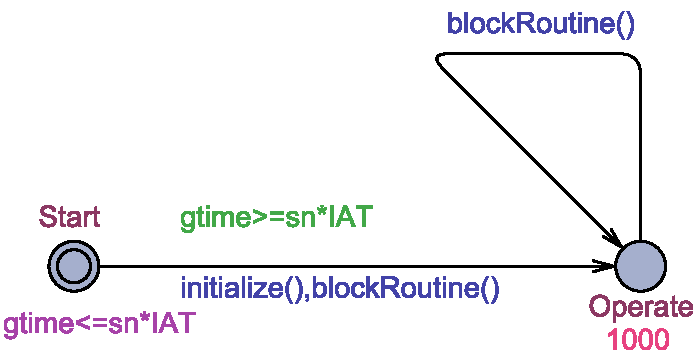
\includegraphics[width=0.9\linewidth]{continuous.pdf}
    \caption{Pattern for Continuous Blocks.}
    \label{fig_continuous_block_ta}
	\end{subfigure}%
	\begin{subfigure}[b]{0.5\textwidth}
  	\centering
  	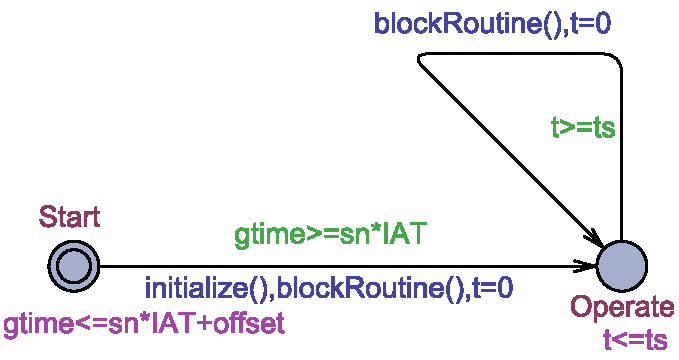
\includegraphics[width=0.9\linewidth]{discrete.pdf}
    \caption{Pattern for Discrete Blocks.}
    \label{fig_discrete_block_ta}
	\end{subfigure}%
  \caption{Our Proposed Timed Automata Patterns.}
  \label{fig_ta}
\end{figure}
\begin{figure}[h]
\centering
\includegraphics[width=\textwidth]{bbw}\\
\caption{The Brake-By-Wire Simulink Model.}
\label{fig_bbw}
\end{figure}



%Simulink is frequently used in the automotive industry to model and simulate the dynamics of automotive functions. Especially for complex automotive systems and stringent functional safety and quality analysis requirements, early analysis is crucial before code generation. In real-time safety critical systems, timing analysis is vital besides functional correctness in order to assure predictability of the system. 

In this contribution, the framework presented in Figure \ref{fig_simulink_modelchecking} relies on two contributions: the SIMPPAL approach and tool for statistical model checking of large Simulink models \cite{Filipovikj2016SimulinkSystems}, validated on two industrial use cases, and its integration with ReSA [the soon-to-be SIMPPAAL meets ReSA paper], which automates requirements specification and their transformation to WMTL properties.In the following, we first explain the SIMPPAAL approach, after which we complete the picture with a short overview of the SIMPPAAL-ReSA integration. 
\begin{figure}[h]
  \centering
  \includegraphics[trim=0 0.75cm 0 0.75cm,clip, width=0.9\linewidth]{modelchecking.pdf}
  \caption{Our Integrated Framework for Model-checking Simulink Models.}
  \label{fig_simulink_modelchecking}
\end{figure}

SIMPPAAL takes input the Simulink model and the sorted execution order of blocks, generated by Simulink, and it transforms the former into a network of stochastic timed automata on which we apply UPPAAL SMC for statistical model checking against properties expressed in WMTL. We use a pattern-based encoding, in which continuous-time Simulink blocks are modeled by instantiating the pattern of Figure \ref{fig_continuous_block_ta}, and discrete-time ones by instantiating the pattern of Figure \ref{fig_discrete_block_ta}. Our pattern-based approach is summarized by the following steps: 

%we propose a formal technique to analyze large and complex  (or industrial) multirate Simulink models via statistical model checking. Figure \ref{fig_simulink_modelchecking} illustrates the model checking which takes in a Simulink model and ReSA specifications, respectively transformed into a network of stochastic timed automata (NSTA) and weighted metric temporal logic (WMTL$\leq$) properties, before invoking the statistical model-checker UPPAAL SMC. 

\begin{itemize}
    \item Step 1: We identify the most frequently-used Simulink blocks by analyzing automotive uses cases from obtained from VGTT and Scania. In order to cover as many blocks as possible,  we investigate several Simulink models that relate chassis control, engine control, and adaptive driver assistance systems.
    \item Step 2: We classify the blocks into continuous and discrete blocks based on their timing execution behavior. The continuous blocks execute over infinitely-small intervals of time and the discrete blocks execute periodically with the sample time $t_s$.
    \item Step 3: We generalize the blocks as tuple $B = \langle V_{in}, V_{out}, V_D, t_s, Init, blockRoutine \rangle$, where: $V_{in}$, $V_{out}$, $V_D$,  are the sets of input, output, data variables, respectively, $t_s$ the a sample time, $Init$ is the initialization function, and $blockRoutine$ is the function that maps input and data variables to output variables.
    %\item Consequently, for the continuous blocks and discrete blocks, we have proposed continuous timed automata (Figure \ref{fig_continuous_block_ta}) and discrete timed automata (Figure \ref{fig_discrete_block_ta}) patters.
    \item Step 4: we propose a transformation that converts the multirate Simulink model into a network of stochastic timed automata via the proposed automata patterns.
    % \begin{itemize}
    % \item if the Simulink model contains compositional blocks, they are flattened first into their constituent atomic Simulink blocks.
    % \item the execution order of the Simulink blocks is preserved in the transformation by employing the Simulink \textit{Sorted Order} list, which states the order in which the blocks are executed, and the list is obtained after simulation of the respective model in the debug mode.
    % \end{itemize}
    \item Step 5: Finally, we statistically model check the network of stochastic timed automata against properties specified in the WMTL$_{\leq}$ temporal logic. We check for probability estimation (in which we calculate the probability of some property to hold), as well as for hypothesis testing, in which we verify that a probability to meet some temporal property is higher than a threshold. 
\end{itemize}

The approach is automated in the SIMMPPAL tool, which is accessible from Bitbucket site \footnote{https://bitbucket.org/predragf/simppaal/src/master/}. Our approch as well as the tool is validated on the Brake-By-Wire industrial Simulink model, shown in Figure \ref{fig_bbw}. The model contains 320 Simulink blocks of which 129 are discrete blocks and 26 are continuous blocks, and the rest are constant blocks. The model is checked against requirements that are translated into WMTL$\leq$ properties \cite{Filipovikj4714}. For each properties, the probability of satisfying the requirement, the confidence of the result and other statistics are returned from the model checker. In contrast to exact model checking, the statistical model checking has not experienced state-space explosion, as expected, for the particular case of the Brake-By-Wire model. In conclusion, the result indicates high confidence values in the range $[0.99-1]$ on average, which is good enough for many embedded systems applications. However, the confidence value can be higher by increasing the number of traces, which has great importance for safety-critical embedded systems applications.

Since the WMTL$\leq$ logic is difficult to use for most engineers, we provide an interface via the ReSA language, which requires extending the ReSA grammar with probabilistic constructs, as well as interpretation of a subset of the ReSA strings according to the WMTL$\leq$ semantics. This work is in progress and is found in Paper F.

We automate the transformation from the Simulink model to the NSTA model in the tool SIMPPAAL, which is accessible from Bitbucket site {\small https://bitbucket.org/predragf/simppaal/src/master/}. Furthermore, we automate the transformation from ReSA to WMTL$_\leq$ [Paper F] transformation from ReSA Our method of transformation as well as the tool is validated on the industrial Brake-By-Wire Simulink model, which is obtained from VGTT. 

% \subsubsection{Contribution 7 - ReSA Toolchain Validation by Practitioners}
% The proposed ReSA toolchain is validated by practitioners from VGTT \footnote{Work in progress}. The main objective of the validation is to evaluate the usability and effectiveness of the proposed methods and tools in practice. The validation of software methods and tools, in general, is challenging in industry mainly because: i) a lot of effort is needed to improve the tools' interface such that it becomes appealing to the evaluators (or practitioners), ii) the process could be stagnant due to practitioners underprioritizing the validation tasks, and iii) it involves a lot of quantitative and subjective data that could lead to inaccurate generalizations.
% \begin{figure}[h]
%   \centering
%   \includegraphics[trim=0 0 0 0,clip,width=0.7\textwidth]{pics/evaluation_process.pdf}
%   \caption{Evaluation Process.}
%   \label{fig_validation}
% \end{figure}

% The evaluation process consists of preparation, data collection and analysis as illustrated in Figure \ref{fig_validation}. It is lead by an evaluation team, which comprises people from MDH and VGTT. Furthermore, it is conducted at the VGTT premises with practitioners and experts in the field, who are selected from different departments of the electrical and/or electronic systems divisions at VGTT such as requirements engineering, system design, software development and verification. As the figure shows, the process begins from preparation of materials such documentation and tutorial for the group such that it prepares them for the actual evaluation. The evaluation data is collected when the participants use the toolchain by observation, during interview after the practice and from a questionnaire. The evaluation team analyzes the data collected and concludes. Afterwards, generalizations are made by inferring the experiences learned from this evaluation process as well as from other related studies on validation of software methods and tools.  



\section{Research Methodology}
\label{section:methods}
\label{methods}
Research methods, according to Jane et al. \cite{qualitateiveresearch2012}, are approaches, procedures and guidelines that are applied to conduct research, e.g., observation, interview, prototyping, experiment, etc. In this research, two main factors have driven the selection of research methods: i) the fact that the research is applied in industry (or involves industry-academia collaboration), which means the research results as well as the process should consider the interest and the nature of the industry, and ii) seamless integration of formal methods into existing engineering methods and practices with minimal cost, which requires careful consideration of existing engineering methods, guidelines, tools and capabilities. To summarize the main problems raised by the industry-academia collaboration: i) the research goals should target existing problems in the industry; ii) existing methods and tools should be leveraged; iii) proposed ideas, methods and tools should be agreed by both academia and industry teams before their design, implementation, validation, and integration to ensure usefulness; iv) furthermore, it is imperative that the proposed tools and methods are engineering-friendly, which means the research team is required to communicate with the actual users to capture the feel of the proposed methods and tools. 
\begin{figure}[h]
\centering
  	\includegraphics[trim=10 0 10 0, clip,width=0.8\linewidth]{pics/research_process.pdf}
    \caption{Research Process.}
    \label{fig_research_process}
\end{figure}

Figure \ref{fig_research_process} illustrates the research process employed in the thesis, which is an adaptation of the technology-transfer process proposed by Tony et al. \cite{Gorschek2006APractice}. Our main research activities has involved identification of research goals and research challenges, which are followed by solution proposals and their implementations. Subsequently, the solutions are validated on industrial use cases, and are also integrated seamlessly into industrial tool chains. In order to conduct these activities, several quantitative and qualitative research methods are blended in order to gather, analyze and interpret, respectively, quantitative and qualitative data via what is known as \textit{hybrid (or mixed) research} \cite{Creswell2014ResearchApproaches}. The benefit of applying mixed research methods is mainly in the triangulation of research outcomes through various research methodical approaches. In fact, this can be better explained by the requirements specification research problem, which has accommodated empirical research via interview, observation to collect quantitative data that has allowed us to understand the current practices and needs of VGTT. Subsequently, we have proposed the ReSA framework, which have been validated through quantitative methods including statistical analysis and questionnaire on its effectiveness and usability\footnote{Work in progress - validation of the ReSA toolchain by practitioners, at VGTT.}.

During implementations of the proposed solutions, we have applied a prototyping method \cite{Carr2004PrototypingApproaches}, which has enabled incremental development of the solutions, before introducing grand progress in subsequent development phases, via concept modeling, implementation, demonstration and revision. This has been the case during the implementation of the ReSA framework \cite{resatool,Mahmud2017SpecificationLogic} as well as the SIMPPAAL framework \cite{Filipovikj2016SimulinkSystems}. The prototyping has involved concept development, and experimentation with toy examples and use cases to internally validate the implementation solutions, before validation by practitioners. Of course, the implementation of the research process has not been straightforward; on the contrary, similar to other research activities, it has accommodated several iterative, cyclic activities to clarify research goals and update solutions based on knowledge gained via literature study and feedback from industry.  Besides, the industrial flavor of the research has required persistent synchronization meetings through discussions and workshops in order to update to the state-of-the-art and state-of-the-practice methods and tools.
% \begin{figure} 
% \centering
  
%   	\includegraphics[trim=20 0 20 0, clip, width=0.7\linewidth]{research_method_activity.pdf}
%     \caption{Activity Diagram of the Research Process.}
%     \label{fig_discrete_block_ta}
%   \label{fig_ta}
% \end{figure}


\section{Thesis Outline}
\label{section:outline}
The thesis is a collection of papers and its outline is presented as follows:

\begin{enumerate}[I]\bfseries
\item Thesis
	\begin{enumerate}[1]
		\item Introduction
		\item Preliminaries
		\begin{enumerate}[2.1]\mdseries
			\item Requirements Specification Methods
            \begin{enumerate}
              \item Template-based Methods
              \item Controlled Natural Language
              \item Formal Specification Methods
            \end{enumerate}
			\item Boolean Satisfiability Problem
			\item Ontology
			\item Software Allocation and Mathematical Optimization
			\item Simulink
			\item Stochastic Timed Automata and UPPAAL Statistical Model Checker (SMC) 
			
		\end{enumerate}
    		\item Research Goals
    		\item Research Method
    		\item Thesis Contributions
		    \begin{enumerate}[5.1]\mdseries
    			\item The ReSA Language
    			\item Formal Semantics of the ReSA Language
    			\item ReSA Framework - Integrated Framework for Formal Analysis of Requirements Specifications
    			\item Optimal Allocation of Multi-rate Distributed Applications
    			\item Formal Analysis of Multi-rate Simulink Models
		    \end{enumerate}
		\item Related Work		
		\item Conclusions and future work
	\end{enumerate}
\item Included Papers
	\begin{enumerate}[1]
		\item Paper A
		\item Paper B
		\item Paper C
		\item Paper D
		\item Paper E
		\item Paper F
	\end{enumerate}
\end{enumerate} 
\pagebreak

\section{Progress and Time Plan}
\label{section:progress}
\subsection{Courses}\vspace{-0.2cm}
The PhD degree requires 75 ECTS from the courses credit which is met as shown in Table \ref{tbl_courses}.
\vspace{-0.2cm}
\begin{table}[h]
	\renewcommand{\arraystretch}{1.3}
	\begin{tabularx}{\textwidth}{|X|p{15mm}|p{18mm}|}
		\hline \rowcolor{gray!10}
		\textbf{Courses} & \centering\arraybackslash \textbf{Credits} & \centering\arraybackslash \textbf{Status} \\
		\hline
		Individual Project & \centering\arraybackslash7.5 & \centering\arraybackslash Finished \\
		\hline
		VeriSpec Project: ReSA Toolchain Integration into AREATOP IDE, VGTT & \centering\arraybackslash7.5 & \centering\arraybackslash Finished \\
		\hline
        Advanced Component-based Software Engineering & \centering\arraybackslash7.5 & \centering\arraybackslash Finished \\
		\hline
		Research Planning & \centering\arraybackslash4.5 & \centering\arraybackslash Finished \\
		\hline
		Research Methods & \centering\arraybackslash7.5 & \centering\arraybackslash Finished \\
		\hline
		Advanced Validation and Verification  & \centering\arraybackslash7.5 & \centering\arraybackslash Finished \\
		\hline
		Principles of Cyber-physical Systems  & \centering\arraybackslash7.5 & \centering\arraybackslash Finished \\
		\hline
		Safety Critical Systems Engineering  & \centering\arraybackslash7.5 & \centering\arraybackslash Finished \\
		\hline
		Project Management and research commercialization  & \centering\arraybackslash 7.5 & \centering\arraybackslash Finished \\
		\hline
	  %  Introduction to Graduate Education for new PhD students  & \centering\arraybackslash 4.5 & \centering\arraybackslash Finished \\
	%	\hline
	    Industrial Systems Cloud Computing  & \centering\arraybackslash7.5 & \centering\arraybackslash Finished \\
		\hline
        International Summer School Marktoberdorf, July 29 to August 10, 2014 & \centering\arraybackslash3.0 & \centering\arraybackslash Finished\\
        \hline
      %  Fourth Summer School on Formal Techniques May 19 - May 23, 2014 Menlo College, Atherton, CA &\centering\arraybackslash2.0 & \centering\arraybackslash Finished\\
        %\hline
       % PhD visit &\centering\arraybackslash 1.0 & \centering\arraybackslash Finished\\
      %  \hline
		\textbf{Total Credits} & \centering\arraybackslash \textbf{75} & \\
		\hline
	\end{tabularx}
	
	\caption{List of Courses Taken.}\vspace{-0.2cm}
		\label{tbl_courses}
\label{coursestble}
\end{table}

\subsection{Time Plan}\vspace{-0.2cm}
The time plan from the beginning of October to the time the PhD thesis is defended is shown as follows:\\[6pt]
 %\tikzset{png export}
\resizebox{1\textwidth}{!}{

    \begin{tikzpicture}
    
    \def\totalmonths{9}
    \def\timelinewidth{18}
    \pgfmathsetmacro\tunit{\timelinewidth/\totalmonths}
    
    % Paper F
    \def\wkPE{8}% working weeks
    \def\offPE{2}
    \def\wkPES{6}% submission week
    \def\wkPEN{16}% notification week
    
    % Paper D
    \def\wkPG{6}% working weeks
    \def\offPG{0}
    \def\wkPGS{8}% submission week
    \def\wkPGN{10}% notification week
    
    % Paper E
    \def\wkPDN{5}% notification week
    
    \def\wkVisit{8}% number of weeks
    \def\wkVisitOff{12}% number of weeks
    \def\wkThesis{12}% number of weeks
    \def\wkThesisOff{16}% number of weeks

    \newcommand{\fWk}[1]
    {
      { #1*\scl}
    }
    \newcommand{\calcx}[2]
    {
      { #1*\tunit + #2*\tunit/4}
    }
    \newcommand{\radius}[1]
    {
      {#1*\tunit/2/4}
    }
    \newcommand{\offset}[2]
    {
      {#1*\tunit/4 + #2}
    }
    \newcommand{\legend}[3]
    {
      { 
         \draw[color=black, dash pattern=on 3pt off 3pt, ultra thick, ->] ({#1},-\radius{#2}-1, 0) -- ({#1},{-\radius{#2}});
         \filldraw[black] ({#1},{-\radius{#2}-1}) circle (2pt) node[anchor=east] {#3};
      }
    }
    \newcommand{\legendNotification}[5]%
    {
      { 
        \draw[color=red, dash pattern=on 3pt off 3pt, ultra thick, ->] ({#1},{#2+#3}, 0) -- ({#1},{#2+0.5});
         \filldraw[black] ({#1},{#2+#3}) circle (2pt) node[anchor=#5] {#4};
      }
    }
    \newcommand{\legendSubmission}[5]%
    {
      { 
        \draw[color=blue, dash pattern=on 3pt off 3pt, ultra thick, ->] ({#1},{#2+#3}, 0) -- ({#1},{#2+0.5});
         \filldraw[black] ({#1},{#2+#3}) circle (2pt) node[anchor=#5] {#4};
      }
    }
          
   
   
    % Paper D
   \fill[fill=cyan](\offset{\offPG}{\wkPG/4},0) circle (\radius{\wkPG});
   \legend{\offset{\offPG}{\wkPG/4}}{\wkPG}{Writing Paper D};
   
   
   % Paper F
    \fill[fill=magenta, fill opacity=0.6](\offset{\offPE}{\wkPE/4},0) circle (\radius{\wkPE}); 
    %\fill[fill=magenta, fill opacity=0.6](0,0) circle (\radius{\wkPE}); 
    \legend{\offset{\offPE}{\wkPE/4}}{\wkPE}{Writing Paper F};

    % Phd visit
    %\draw[pattern=dots, pattern
    \fill[fill=orange](\offset{\wkVisitOff}{\wkVisit/4}, 0) circle (\radius{\wkVisit});
   \legend{\offset{\wkVisitOff}{\wkVisit/4}}{\wkVisit}{PhD Visit};


   % Thesis writing
    %\draw[pattern=dots, pattern
    \fill[fill=green!70,fill opacity=0.8](\offset{\wkThesisOff}{\wkThesis/4}, 0) circle (\radius{\wkThesis});
    \legend{\offset{\wkThesisOff}{\wkThesis/4}}{\wkThesis}{PhD Thesis Writing};


    %% Notifications
    \legendNotification{\offset{18}{0}}{0}{3}{Paper F Notification (NFM 2019}{east};%(x,y,height, message)
    \legendNotification{\offset{20}{0}}{0}{4}{Paper D Notification (JSS)}{east};
    \legendNotification{\offset{22}{0}}{0}{5}{Paper E Notification (TOSEM)}{east};
    \legendSubmission{\offset{28}{0}}{0}{3}{Send Thesis for Print}{west};
    \legendNotification{\offset{27}{0}}{0}{4}{Paper F Notification (SEKE 2019)}{west};
    \legendSubmission{\offset{34}{0}}{0}{2}{Defend PhD Thesis}{south};
    
    % Draw timeline
    \filldraw[color=red!60, fill=red!5, very thick] (-1,-0.75) rectangle (\timelinewidth,0.5);
    \foreach \x/\y in {0/Oct,1/Nov,2/Dec,3/Jan,4/Feb,5/Mar,6/April,7/May,8/June }
    {       
        \draw (\calcx{\x}{0},3pt) -- (\calcx{\x}{0},-3pt) node[above=3pt] {\y}; 
        \foreach \z in {1,2,3} 
           \draw (\calcx{\x}{\z},3pt) -- (\calcx{\x}{\z},-3pt);
    }
    % \pgfmathsetmacro\resultt{(\j * 2) + 1}
  \end{tikzpicture}}
%\includepdf[pages=-]{thirdcycle.pdf}
\pagebreak

%research area
\subsection{Thesis Opponent and Committee}
For the thesis defense we propose the preliminary committee as follows:
\begin{enumerate}
	\item Opponent: Prof. Joost-Pieter Katoen, RWTH Aachen University, Germany, and University of Twente, the Netherlands
	\item Committee members:
	\begin{enumerate}
		\item Antonia Bertolino, Research Director at CNR, Italy
		\item Associate Professor Patrizio Pellicione, Chalmers University of Technology, Sweden
        \item Professor Peter Csaba {\"0}lveczky, University of Oslo, Norway
      %  \item Professor Einar Broch Johnsen, University of Oslo, Norway
		%\item Assistant Professor Marco Autili, University of  L'Aquila, Italy
	\end{enumerate}
	\item Reserve: To be decided
\end{enumerate}

\section{Third Cycle Outcome}
\label{section:thirdcycle}
%Knowledge and understanding
\rowcolors{2}{gray!25}{white}
\begin{longtable}{|p{0.8\linewidth}|l|}
\hline \textbf{1.~Knowledge and understanding} & \textbf{Completed }\\
\hline
\hline 1.1a~ Knowledge and understanding of the research area & YES\\
\hline \multicolumn{2}{|}{}
  \begin{minipage}{\linewidth}\vspace{0.2cm}
  I have taken the following graduate courses:\vspace{-0.2cm}
  \begin{itemize}\itemsep-0.25em
    \item Advanced component-based software  engineering, 7.5 credits
    \item Research methodology, 7.5 credits
    \item Industrial Systems Cloud Computing, 7.5 credits
    \item Research planning, 3 credits
    \item Dependable Software Systems Engineering, Marktoberdorf Summer School 2014, 3 credits
    \item Advanced Software Verification and Validation, 7.5 credits
    \item Design of Cyber-Physical Systems, 7.5 credits
    \item Safety Critical Systems Engineering, 7.5 credits
    \item Project Management and research commercialization, 7.5 credits
  \end{itemize}
  \end{minipage}\hfill\vline\kern-\arrayrulewidth\\[2cm]
\multicolumn{2}{|}{}
  \begin{minipage}{\linewidth}  \vspace{0.2cm}
 I have attended the following schools, workshops and conferences:\vspace{-0.2cm}
  \begin{itemize}
 \itemsep-0.25em
    \item The 36th IEEE Software Engineering Workshop (SEW-36), Gdansk, Poland, 11-14 September 2016
    \item SIES'2015: 10th IEEE International Symposium on Industrial Embedded System, Siegen, Germany, 8-10 June 2015
    \item IEEE Emerging Technology and Factory Automation (ETFA 2014), Barcelona, Spain, 16-19 September 2014
    \item 21st International Symposium on Formal Methods, limassol, Cyprus,  9-11 November 2016
    \item Federated Conference on Computer Science and Information Systems, Trento, Italy, 4-8 September 2017
  \end{itemize}
  \end{minipage}\hfill\vline\kern-\arrayrulewidth\\[2cm]
  \multicolumn{2}{|}{}
  \begin{minipage}{\linewidth} \vspace{0.2cm}
 I have attended the following webinars, seminars, licentiate and doctoral proposals and presentations:\vspace{-0.2cm}
  \begin{itemize}
  \itemsep-0.25em
  \item licentiate/PhD seminars and presentations
  \item lectures given by guest professors at MDH
  \item seminars in other research groups at MDH
  \item seminar in other places (Volvo VGTT, Scania, SICS Open House, Software Center)
  \end{itemize}
  I have authored and co-authored the following papers:
  \begin{itemize} \itemsep-0.25em
    \item The Multi-Resource Server for Predictable Execution on Multi-core Platforms (Apr 2014) 
    Rafia Inam, Nesredin Mahmud, Moris Behnam, Thomas Nolte, Mikael Sj{\"o}din 
    \item Evaluating Industrial Applicability of Virtualization on a Distributed Multicore Platform (Sep 2014) 
    Nesredin Mahmud, Kristian Sandstr{\"o}m, Aneta Vulgarakis Feljan 
    \item ReSA: An Ontology-based Requirement Specification Language Tailored to Automotive Systems (Jun 2015) 
    Nesredin Mahmud, Cristina Seceleanu, Oscar Ljungkrantz 
    \item ReSA Tool: Structured Requirements Specification and SAT-based Consistency-checking, Nesredin Mahmud, Cristina Seceleanu, Oscar Ljungkrantz

    \item Simulink to UPPAAL Statistical Model Checker: Analyzing Automotive Industrial Systems (Nov 2016) 
    Predrag Filipovikj, Nesredin Mahmud, Raluca Marinescu, Cristina Seceleanu, Oscar Ljungkrantz , Henrik Lönn 
    \item Semantic Analysis of Embedded System Requirements Specifications, Nesredin Mahmud, Cristina Seceleanu, Oscar Ljungkrantz,Technical Report
    \item Specification and Semantic Analysis of Embedded Systems Requirements: From Description Logic to Temporal Logic,
    Nesredin Mahmud, Cristina Seceleanu and Oscar Ljungkrantz
    \item Power-aware Allocation of Fault-tolerant Multi-rate AUTOSAR Applications, Nesredin Mahmud, Guillermo Rodriguez-Navas, Hamid Faragardiy, Saad Mubeen, Cristina Seceleanu
   \item Ontology-based Analysis and Scalable Model Checking of Embedded Systems Models, 
Nesredin Mahmud \\
  \end{itemize}

  \end{minipage}\hfill\vline\kern-\arrayrulewidth\\[2cm]
\hline 1.1b~ Specialist knowledge in a defined part of the research area & YES\\
\hline \multicolumn{2}{|}{}
  \begin{minipage}{\linewidth}\vspace{0.2cm}
  I have taken the following graduate courses:\vspace{-0.2cm}
    \begin{itemize} \itemsep-0.25em
    \item Advanced Validation and Verification, 7.5 
    \item Safety-critical Systems Engineering, 7.5 
    \end{itemize}
   I have visited Volvo Groups Trucks Technology (VGTT), Gothenburg several times.
  \begin{itemize} \itemsep-0.25em
  \item I spent time investigating existing engineering tools, and development methods.
  \item I interviewed senior developers, group managers, and leaders from various departments.
  \item I have conducted empirical study on requirements specification at VGTT.
  \item I have used VGTT automotive use cases to validate our proposed solutions.
  \item I participated in the VGTT department meetings.\\
  \end{itemize}
  \end{minipage}\hfill\vline\kern-\arrayrulewidth\\[2cm]
\hline 1.1c~ Deep knowledge of research methods in general, and of research methods in the specific research area & YES\\
\hline \multicolumn{2}{|}{}
  \begin{minipage}{\linewidth}\vspace{0.2cm}
  I have taken the following graduate courses:\vspace{-0.2cm}
  \begin{itemize} \itemsep-0.25em
    \item Research methodology, 7.5 credits
  \end{itemize}
  Deep knowledge of research methods in general area:
  \begin{itemize} \itemsep-0.25em
  \item research problem solving  in industrial context
  \item embedded systems, cyber-physical research method
  \end{itemize}
  Deep knowledge of research methods in specific area:
  \begin{itemize} \itemsep-0.25em
  \item research solving for improving quality of embedded systems in automotive domain
  \item automotive system design and anlysis method
  \item software evaluation method in automotive domain
  \end{itemize}
  \end{minipage}\hfill\vline\kern-\arrayrulewidth\\[4cm]
\hline   Remaining Activities&\\
\hline \multicolumn{2}{|}{}
\begin{minipage}{\linewidth}\vspace{0.2cm}
  \begin{itemize} \itemsep-0.25em
  \item Writing Paper D
  \item Writing Paper F
  \item Writing PhD thesis
  \end{itemize}
  \end{minipage}\hfill\vline\kern-\arrayrulewidth\\[2cm]
\hline
\end{longtable}

\pagebreak
% Skills and abilities
\rowcolors{2}{gray!25}{white}
\begin{longtable}{|p{0.8\linewidth}|l|}
\hline \textbf{2.~Skills and abilities} & \textbf{Completed}\\
\hline
\hline 2.1a~ Critically and independently identify and formulate research questions & YES\\
\hline \multicolumn{2}{|}{}
  \begin{minipage}{\linewidth}\vspace{0.2cm}
  \begin{itemize}\itemsep-0.25em
    \item I have written scientific articles and papers indicated in 1.1a.
    \item I have written basic and advanced level thesis proposals:\\
    \indent - Automated Transformation of Requirements from Natural language to Formal specification\\
    \indent - Integration of ReSA into an Industrial IDE
    \item I have written my licentiate thesis proposal.
    \item I have written my PhD thesis proposal.
    \item I maintained lab assignments.
  \end{itemize}
  \end{minipage}\hfill\vline\kern-\arrayrulewidth\\

 \hline 2.2b~ Contribute to the development of knowledge & YES\\
\hline \multicolumn{2}{|}{}
  \begin{minipage}{\linewidth}\vspace{0.2cm}
  I contributed research results to research communities, shown in 1.1.a.\\
  I assisted the following labs:
  \begin{itemize}\itemsep-0.25em
     \item Software Development for Real-Time Systems, DVA421 (7.5 credits) in 2017,18
     \item DVA218 vt 2017 Datakommunikation, DVA218 (7.5 hp) in 2015, 16, 17,18
     \item Datakommunikation f{\"o}r inbyggda system I, DVA235 (7.5 credits) in 2016
     \item Project in advanced embedded systems, DVA474, (7.5 credits) in 2015, 16, 17 times)
  \end{itemize}
  I supervised students: \vspace{-0.2cm}
  \begin{itemize} \itemsep-0.25em
    \item master level: \emph{Object Detection For High Productivity, 2015}
    \item master level: \emph{Automated Transformation of Requirements from Natural language to Formal specification, 2016} (Interrupted)
  \end{itemize}
  I contributed research results to industry.
  \end{minipage}\hfill\vline\kern-\arrayrulewidth\\

  \hline 2.2~Orally and in writing present and discuss research results with the national and international scientific community, and the society in general & YES\\
  \hline \multicolumn{2}{|}{}
  \begin{minipage}{\linewidth}\vspace{0.2cm}
  I have attended the following scientific community for seminar, conference, workshop
    \begin{itemize} \itemsep-0.25em
    \item 19th IEEE International Conference on Emerging Technologies and Factory Automation, Barcelona
    \item The 36th IEEE Software Engineering Workshop (SEW-36), Gdansk
    \item Fuse, Joint Seminar on Functional Safety, Virtual Integration and Model Based Engineering, G\"oteborg
    \item I participated in VGTT, Scania s\"odert\"alje workshop, and meetings
    \item Federated Conference on Computer Science and Information Systems, Trento, Italy, 4-8 September 2017
  \end{itemize}
  \end{minipage}\hfill\vline\kern-\arrayrulewidth\\

  \hline 2.3 Independently conduct research and development & YES\\
  \hline \multicolumn{2}{|}{}
  \begin{minipage}{\linewidth}\vspace{0.2cm}
    \begin{itemize} \itemsep-0.25em
    \item As main driver, I have been responsible for research, and publication of the scientific papers listed in Section \ref{papersincl}
    \item I conducted research visits at VGTT, Scania s\"odert\"alje
    \item I have developed research prototypes
    \item I have validated research results on industrial uses cases
    \item I have conducted empirical research at VGTT on requirements specification
    \item I initiated research cooperation on some research topics and have worked with it.
  \end{itemize}
  \end{minipage}\hfill\vline\kern-\arrayrulewidth\\
\hline
\end{longtable}

\pagebreak
% Judgement and approach
\rowcolors{2}{gray!25}{white}
\begin{longtable}{|p{0.8\linewidth}|l|}

\hline \textbf{3.~Judgment and approach} & \textbf{Completed} \\
\hline
\hline 3.1~~Demonstrate ability to make ethical assessments in own research & YES\\
\hline \multicolumn{2}{|}{}
  \begin{minipage}{\linewidth}\vspace{0.2cm}
  I have participated in the planning of my own research\\
  I have taken courses that contributed knowledge to ethical assessments such as:
  \begin{itemize}\itemsep-0.25em
    \item Research Methods Course, 7.5credit
    \item Research Planning Course, 4.5credit
  \end{itemize}
  I have worked together with industrial partners which I have learned individuals and organizational ethics.
  \end{minipage}\hfill\vline\kern-\arrayrulewidth\\

 \hline 3.2 Demonstrate understanding of science's role and use in society, including its possibilities and limitations, and responsibility of its use & YES\\
\hline \multicolumn{2}{|}{}
  \begin{minipage}{\linewidth}\vspace{0.2cm}
  \begin{itemize} \itemsep-0.25em
    \item I participated in co-production with VGTT, Scania
    \item I participated in research projects, in general which had required ethical practices.
  \end{itemize}
  \end{minipage}\hfill\vline\kern-\arrayrulewidth\\

  \hline 3.3 Identify one's need of further knowledge and take responsibility for one's learning & YES\\
  \hline \multicolumn{2}{|}{}
  \begin{minipage}{\linewidth}\vspace{0.2cm}
    \begin{itemize} \itemsep-0.25em
    \item I have authored and co-authored papers listed in 1.1a.
    \item I have participated and presented research results in international venues.
    \item I have participated in seminars and workshops to exchange knowledge.
    \item I have developed software engineering tools, in particular relevant for industry.
    \item I have visited VGTT, Gutenberg to better understand research problems.
    
  \end{itemize}
  \end{minipage}\hfill\vline\kern-\arrayrulewidth\\
\hline
\end{longtable} 


\section{Related Work}
\label{section:related}
In this section are discussed the related work on specification and analysis of requirements, allocation of software architecture, and formal analysis of behavioral models, designed in Simulink.

\subsection{Requirements Specification and Analysis}
Embedded system requirements are captured in different representations, e.g., textual, tabular, graphical, etc. The textual representation, which is the scope of the analysis, can be conveniently classified into two classes: i) controlled natural language (CNL), ii) template-based methods.  The syntax and semantics of the CNLs are similar to natural language except that the lexicon and the syntax are restricted for different reasons, of which improving comprehensibility of the text and formal representations to support rigour analysis of the text are prominent. The ReSA language is designed to improve comprehensibility of requirements specifications as well as to be computer-processable. There are many computer-processable CNL in literature \cite{Kuhn2014ALanguages}, e.g., Attempto Controlled English (ACE) \cite{attempto96}, Processable English (PENG) \cite{Schwitter2002EnglishLanguage}, etc. Similar to most computer-processable languages, ReSA has limited syntactic constructions, and allows knowledge-representations, in contrast though, our language is catered for embedded systems and therefore it uses concepts as well as semantic rules that are domain-specific to embedded systems. Similar to PENG, its implementation supports look-ahead in order to enable predictive and guided specification.

The template-based methods, in particular requirements boilerplate uses templates (or boilerplates) which are reusable, recurrent patterns to specify requirements, e.g., CESAR boilerplates \cite{Farfeleder2011DODT:Development}, RAT, etc. The main drawback of existing requirements boilerplates are: i) the templates are usually too limited therefore not expressive enough, ii) it is not easy to find the appropriate boilerplate during specification. In this regard, ReSA extends boilerplates with a meta-model that guides for plausible instantiation of boilerplates.

\subsection{Optimal Allocation of Software Architectures}
Different allocation schemes deliver different system performance and therefore efficient software allocation is crucial. Ernest Wozniak et al. \cite{Wozniak2013AnArchitectures} proposed a synthesis mechanism for an AUTOSAR software application that can executed over multiple nodes, with the objective fulfilling timing requirements. In contrast, we consider power consumption and reliability requirements besides timing. Similarly, Salah Saidi et al. \cite{Saidi2015AnArchitectures} proposed an ILP based approach for allocation of an AUTOSAR application on a multi-core framework in order to reduce the overhead of inter-process communication while we consider a multi-nodes platform. Ivan Svogor et al. \cite{vsvogor2014extended} proposed a generic approach of identifying resource constraints and a way of handling different measurement units with Analytic Hierarchy Process (AHP) in order to allocate a component-based software application on a heterogeneous platform. However, the resource constraints are trivialized, e.g., end-to-end delay calculations, which require timing specifications and activation patterns of tasks. As opposed to the previously mentioned related work, we considered a system model with a multi-rate software application, which basically impose complex timing analysis due to complex timed paths from the source to the sink of communication signals \cite{mubeen2013support}. On a different work, there are research focusing on power and energy consumption in real-time distributed systems which are employ dynamic voltage scaling ~\cite{bambagini2016energy} and task consolidation by minimizing computational nodes ~\cite{faragardi2013towards}~\cite{devadas2012interplay}.

\subsection{Formal Analysis of Simulink Models}
Several research endeavors have tackled the problem of formally analyzing Simulink models in order to gain better insight into the design of Simulink model, and they mainly differ in the aspects (or coverage) of the Simulink language that has been targeted for analysis and the formalisms applied. Besides to the scalability of the techniques, their robustness to formally analyze various types of Simulink models is also crucial especially for the proposed methods to be useful in industry. In this related work on formal analysis of Simulink models, existing formalisms and their applicability in industry are discussed, and also compared to our solutions.

Simulink already suppors formal analysis of Simulink models via its Simulink Design Verifier (SDV) product\footnote{https://se.mathworks.com/products/sldesignverifier.html}. Though, there is limited resource to investigate about the pros and cons of the product, the study by Nellen et al. \cite{Nellen2018FormalRecommendations} indicates some limitations on its capability such as inconclusiveness on the verification results, lack of support to verify timed properties. The latter pros is also mentioned by Florian et al. \cite{Leitner2008SimulinkStudy} in the comparison against SPIN. For brevity, other approaches are classified into three categories, approaches that use Simulink traces, contract/theorem and model-to-model transformation. 

The PlasmaLab proposed by Nikolaos et al. \cite{Kekatos2018ConstructingHybridization} transforms Simulink sample traces into statistical models, which are eventually analyzed by their statistical mode checker. Albeit the checker is assisted by an algorithm that determines sufficiency of the sample traces, it is unclear how it works. Unlike many approaches, PlasmaLab can analyze any Simulink models as long as the simulation results sample trances, which is the main advantage. Ferrante et al. \cite{Hocking2016ProvingModels} use contract-based theory in order to lift the block specification, and rely on a combination of SAT solvers and the NuSMV model checker for analysis. Hocking et al. \cite{Ferrante2012ParallelSystems} use the PVS specification language for writing the specification, and rely on the PVS theorem prover for analysis. A limitation of this strategy is that both steps still require much user interaction, so it is error-prone and requires certain understanding of the formal analysis engines, which is not common among embedded systems engineers.

The model-to-model transformation approach basically transforms the Simulink model into a formal model that can be checked via model checking, e.g., for reachability properties. Bernat et al. \cite{Meenakshi2006ToolChecker} proposed transformation Simulink models that consist only discrete blocks, which are subsequently checked via the DiViNE model checker. The research endeavors proposed transformation only StateFlow/Simulink into timed and hybrid automata. The discussed model-to-model approaches are limited in scalability due the use of exact model checking. In contrast, our approach uses statistical model checking, and thus scales better albeit is not exhaustive. However, by collecting sufficient sample traces and consequently acceptable confidence value in the statistical analysis, the later challenge can be tackled. Furthermore, our approach supports transformation of any discrete and continuous blocks, and also blocks that are custom and StateFlow. The latter capability is achieved since our transformation abstracts the internal implementation of the blocks.



%lack of soto not be incontBarnat et al. \cite{Barnat2012ToolDesigns} and Meenakshi et al. \cite{Meenakshi2006ToolChecker} propose transformations that target only Simulink blocks with discrete-time behavior. The work of Agrawal et al. \cite{agrawal2004semantic} focuses on the transformation of Simulink into networks of automata, without providing concrete means for formal verification. Miller \cite{miller2009bridging} investigates how translating Simulink to Lustre enables formal verification with a constellation of model checkers and provers. Manamcheri et al. \cite{Manamcheri2011AModels} and Jiang et al. \cite{Jiang2018DependableCPS} propose transformation frameworks for Stateflow diagrams, into timed and hybrid automata, respectively, yet not considering other types of Simulink blocks. Compared to these frameworks, our approach covers both continuous- and discrete-time blocks, and we show how our transformation leads to the formal analysis of industrial automotive systems models, against a wide set of requirements. This is an endeavor not really carried out before. One other solution is the use of PLASMA Lab \cite{Legay2016StatisticalLab}, a tool that is able to take as input different Simulink simulations and provide statistical model checking results. Compared to this approach, we generate a formal model that can be extended further (e.g., with extra-functional information) to provide additional verification results. 

\section{Conclusions and Future Work}
\label{section:conclusions}
Improving functional safety and quality of embedded systems is crucial due to the catastrophic consequences of their failure. Besides their applications in ragged environment, operating for a along time without interruption and the fact that such system are usually resource constrained, call for a systematic development approach. In this thesis, we have proposed several formal techniques for improving functional safety and quality of embedded systems, including requirements specifications, software system architecture, and software behavior, modelled in Simulink.

We proposed a domain-specific language for the specification of embedded systems requirements called ReSA. The language resembles the natural language English in syntax and semantics. However, its syntax is constrained in order to improve comprehensibility of the specifications. The language has formal semantics in Boolean and description logic, which has enabled for superficial and deep analysis of the requirements, e.g., consistency checking. The ReSA toolchain contains a ReSA editor that supports content-completion to guide requirements specification, and the specifications can be checked for consistency via the Z3 SMT solver. The language is validated for its expressively on a set of 300 industrial requirements, and has proven to express about 90\% of the requirements. 

We have also provided a mechanism to preserve timing and reliability requirements of multirate software applications during software allocation, while minimizing power consumption via Integer Linear Programming, ILP (exact) and Particle Optimization, PSO (meta-heuristic) methods. The ILP method is shown to be applicable to allocation of small and medium of software applications, whereas the PSO has shown to scale well for allocation of large software applications.

Furthermore, we have introduced an automated pattern-based, order-preserving method for transforming behavioral embedded systems models in Simulink into networks of stochastic timed automata analyzable by UPPPAAL SMC. The method is implemented in our tool SIMPPAAL that we have integrated with ReSA and validated on the BBW industrial prototype. 

The ReSA language is a descriptive and intuitive language as it resembles natural language. By extending its constructs to encompass design constraints, it should be possible and in fact beneficial to synthesize a high-level architecture, using correct-by-construction. Furthermore, by raising detailed hardware platform specifications in to the system design, e.g., memory, CPU, power specification, effective software to hardware allocation can be achieved. The proposed formal analysis of Simulink models can be generalized to other language that comply to a data-flow programming paradigms, e.g., LabView. 


%\nocite{*}
\bibliographystyle{plain}
\bibliography{proposal}

\end{document}

